\chapter{Implementazione}\label{cap:implementazione}
\section{Setup}
Prima di passare all'implementazione vera e propria della piattaforma \`e necessario configurare tutti gli strumenti che verranno utilizzati per il suo sviluppo.
\subsection{Laravel}
\subsubsection{Database}
Per connettere il database MySQL all'applicazione Laravel si dovranno specificare i dettagli del server MySQL (host, porta, nome del database, etc.) all'interno del file di configurazione \verb|config\database.php|. Laravel fornisce un supporto first-party per i database MySQL, quindi, sar\`a  necessario inserire solamente le informazioni per la configurazione sotto la voce \verb|mysql| dell'array \verb|connections|~\cite{LaravelDBConfig}. 
\subsubsection{Storage}
Per configurare il filesystem in modo tale che i file caricati dagli utenti siano pubblicamente accessibili \`e necessario configurare i driver di archiviazione e la posizione di archiviazione specificati nel file di configurazione \sloppy\verb|config\filesystems.php|.

Come driver di archiviazione verr\`a utilizzato il driver locale, ossia il driver che interagisce con i file archiviati localmente sul server che esegue l'applicazione Laravel. Per rendere questi file accessibili dal web, \`e necessario creare un collegamento simbolico. Per fare ci\`o si esegue il comando Artisan~\cite{LaravelFilesystemConfig}:
\begin{lstlisting}[basicstyle=\linespread{1.4}\ttfamily\fontsize{11pt}{11pt}\selectfont]
php artisan storage:link
\end{lstlisting}
\subsubsection{E-mail}
Per permettere all'applicazione di inviare e-mail si dovranno specificare i dettagli del server SMTP (host, porta, etc.) all'interno del file di configurazione \verb|config\mail.php|. Laravel fornisce nativamente i driver per l'invio di e-mail tramite SMTP, quindi, sar\`a  necessario inserire solamente le informazioni per la configurazione sotto la voce \verb|smtp| dell'array \verb|mailers|~\cite{LaravelEmailConfig}. 
\subsubsection{Template delle e-mail}
Per personalizzare il template delle e-mail inviate tramite Laravel \`e necessario esportare i componenti attraverso il comando Artisan:
\begin{lstlisting}[	basicstyle=\linespread{1.4}\ttfamily\fontsize{11pt}{11pt}\selectfont]
php artisan vendor:publish --tag=laravel-mail
\end{lstlisting}
Tale comando pubblicher\`a i componenti mail nella cartella \verb|resources\views\vendor\mail|. La cartella \verb|mail| conterr\`a, a sua volta, una cartella HTML e una di testo, ciascuna contenente le rispettive rappresentazioni di ogni componente disponibile~\cite{LaravelEmailConfig}.

\subsubsection{Verifica dell'indirizzo e-mail}
Per la verifica dell'indirizzo e-mail, il modello \verb|User| deve implementare il contatto \verb|Illuminate\Contracts\Auth\MustVerifyEmail|~\cite{LaravelEmailVerification}.

L'e-mail che verr\`a inviata all'utente viene definita attraverso una chiusura passata come parametro al metodo \verb|toMailUsing| della classe \verb|Illuminate\Auth\Notifications\VerifyEmail| nel metodo \verb|boot()| della classe \verb|App\Providers\AuthServiceProvider|.

Per proteggere le route dagli utenti che non hanno verificato la propria e-mail \`e disponibile il middleware ``verified'', fornito dalla classe \verb|Illuminate\Auth\Middleware\EnsureEmailIsVerified|~\cite{LaravelEmailVerification}.

\subsubsection{Reimpostazione delle password}
Per reimpostare la password, il modello \verb|User| deve utilizzare il trait \verb|Illuminate\Auth\Passwords\CanResetPassword|~\cite{LaravelResetPassword}.

L'e-mail che verr\`a inviata all'utente viene definita attraverso una chiusura passata come parametro al metodo \verb|toMailUsing| della classe \verb|Illuminate\Auth\Notifications\ResetPassword| nel metodo \verb|boot()| della classe \verb|App\Providers\AuthServiceProvider|.

\subsubsection{Policy}
Le policy sono classi che permettono di gestire la logica di autorizzazione per un modello o una risorsa. Tutte le policy del progetto vengono registrate all'interno della propriet\`a \verb|policies| della classe \sloppy\verb|App\Providers\AuthServiceProvider|\allowbreak~\cite{LaravelPolicy}.

Per questo progetto sono state utilizzate due policy \verb|UserPolicy| e \verb|PortfolioPolicy| presenti nella cartella \verb|App\Policies\v1|.

\subsubsection{Sanctum}
Sanctum \`e preinstallato in ogni progetto Laravel e per essere utilizzato \`e necessario aggiungere il suo middleware al tuo gruppo di middleware \verb|api| all'interno del file \verb|app\Http\Kernel.php|~\cite{LaravelSanctumConfig}:
\begin{lstlisting}
'api' => [
	\Laravel\Sanctum\Http\EnsureFrontendRequestsAreStateful::class,
	...
],
\end{lstlisting}

Per utilizzare i meccanismi di autenticazione di Sanctum \`e necessario, inoltre, configurare il file di configurazione \verb|config\auth.php|. In tale file \`e possibile configurare il driver di autenticazione dell'API in modo tale che utilizzi Sanctum:
\begin{lstlisting}[basicstyle=\ttfamily\fontsize{9pt}{9pt}\selectfont]
'guards' => [
	...
	'api' => [
		driver' => 'sanctum',
		...
	],
],
\end{lstlisting}

Per la generazione dei token Sanctum il modello \verb|User| deve utilizzare il trait \verb|Laravel\Sanctum\HasApiTokens|~\cite{LaravelSanctumConfig}.


\subsubsection{Risposte JSON}
Per implementare le risposte secondo lo standard JSend \`e stato sviluppato il trait PHP \verb|App\Traits\JSONResponse| che mette a disposizione i metodi \verb|successResponse|, \verb|failResponse| e \verb|errorResponse| per gestire le risposte di successo, fallimento ed errore, rispettivamente.
\subsubsection{Soft delete}
Per poter ripristinare l'account utente, il portfolio e le gallerie dopo essere stati eliminati, i modelli \verb|User|, \verb|Portfolio| e \verb|Gallery| devono utilizzare il trait \verb|Illuminate\Database\Eloquent\SoftDeletes|~\cite{LaravelSoftDeleting}.

\subsubsection{Routing}
Le route Laravel vengono definite nei file presenti nella cartella \verb|routes| i quali devono essere caricati nel metodo \verb|boot()| della classe \sloppy\verb|App\Providers\RouteServiceProvider|~\cite{LaravelRoute}.

In questo progetto sono presenti tre file di route:
\begin{itemize}
	\item \verb|routes\api\auth.php|: contenente le route per implementare le fasi di autenticazione.
	\item \verb|routes\api\v1\api.php|: contenente le route principali della piattaforma.
	\item \verb|routes\api\v1\cms.php|: contenente le route per la gestione del contenuti nei portfolio.
\end{itemize}

\begin{lstlisting}
$this->routes(function () {
	Route::middleware('api')
		->prefix('auth')
		->group(base_path('routes/api/auth.php'));
	
	Route::middleware('api')
		->prefix('v1')
		->group(base_path('routes/api/v1/api.php'));
	
	Route::middleware(['api', 'auth:api', 'verified'])
		->prefix('v1/cms')
		->group(base_path('routes/api/v1/cms.php'));
});
\end{lstlisting}

\subsection{Vue.js}
\subsubsection{Axios}
Axios \`e una libreria JavaScript utilizzata per effettuare e gestire richieste HTTP. Per fare ci\`o, lato server utilizza il modulo nativo \verb|http| di \verb|node.js|, mentre lato client utilizza le \verb|XMLHttpRequests|~\cite{Axios}.

Una volta installato, attraverso il comando \verb|npm install axios|, per utilizzarlo \`e stato creato un file di configurazione denominato: \verb|axiosConfig.js|. In tale file viene specificato il \verb|baseURL| il quale punta all'indirizzo al quale \`e presente l'API della piattaforma. Inoltre \`e necessario configurare gli \verb|interceptors| i quali permettono di intercettare richieste e risposte prima che esse vengano gestite. Per ogni richiesta, se l'utente \`e autenticato alla piattaforma, \`e necessario impostare il campo \verb|Authorization| dell'header con l'access token dell'utente. Per ogni risposta invece, se il codice di stato \`e \verb|401|, si esegue la disconnessione dell'utente dalla piattaforma, mentre se il codice di stato \`e \verb|403| l'utente viene reindirizzato alla pagina ``/not-found''.
\subsubsection{Vue Router}
Vue Router \`e il router ufficiale per Vue.js. Vue Router permette di realizzare una navigazione fluida tra le diverse pagine di una SPA.

Una volta installato, attraverso il comando \verb|npm install vue-router@4|, si definisce la struttura di navigazione delle pagine nel file: \verb|router\index.js|.

Il router viene installato nell'applicazione come plugin. Per fare ci\`o, viene importato il router nel file \verb|main.js|, nel quale viene creata l'applicazione Vue.js, e installo attraverso il metodo \verb|use|.
\subsubsection{Pinia}
Una volta installato Pinia, attraverso il comando \verb|npm install pinia|, viene installato come plugin dell'applicazione Vue.Js. Ogni store verr\`a poi definito nella cartella \verb|store|.

\subsubsection{Tailwind CSS}
Una volta installato Tailwind CSS, attraverso il comando \verb|npm install -D tailwindcss postcss autoprefixer|, occorre generare i file di configurazione \verb|tailwind.config.cjs| e \verb|postcss.config.cjs| attraverso il comando \verb|npx tailwindcss init -p|. Infine, per utilizzare il framework, \`e necessario includere le seguenti direttive Tailwind al file CSS principale dell'applicazione \verb|index.css|:
\begin{lstlisting}
@tailwind base;
@tailwind components;
@tailwind utilities;
\end{lstlisting}

\section{Autenticazione}
L'implementazione dell'autenticazione consiste, principalmente, nella realizzazione di tutte le componenti necessarie per la registrazione di un nuovo utente e per la gestione dell'accesso e disconnessione dalla piattaforma.
\subsection{Registrazione}
\subsubsection{Laravel Route}
Per implementare la registrazione alla piattaforma sono state definite tre route nel file \verb|routes\api\auth.php| (Codice~\ref{lst:route_registration}).
\begin{lstlisting}[caption={Route per la registrazione}, label={lst:route_registration}]
Route::post('register', [RegisteredUserController::class, 'store']);
Route::get('email', [EmailController::class, 'show']);
Route::get('username', [UsernameController::class, 'show']);
\end{lstlisting}

La prima gestisce la fase di creazione di un nuovo utente, mentre le altre due permettono di verificare la disponibilit\`a, rispettivamente, di un indirizzo e-mail e uno username.

\subsubsection{RegisteredUserController@store}
Il metodo \verb|store| della classe \verb|RegisteredUserController| ha come unico parametro una richiesta di tipo \verb|RegisteredUserRequest|. La classe \verb|RegisteredUserRequest| si occupa di convalidare ogni richiesta, verificando che siano presenti i campi ``username'', ``name'', ``email'', ``password'' e ``password\_confirmation'', necessari per effettuare la registrazione e che rispettino le regole definite nella classe \verb|Rules|.

Se la richiesta \`e valida viene eseguito il metodo, il quale:
\begin{itemize}
	\item Crea un nuovo utente nella base di dati.
	\item Crea una foto profilo utilizzando le iniziali del nome dell'utente.
	\item Crea un token Sanctum.
	\item Invia una e-mail per la verifica dell'indirizzo e-mail.
\end{itemize} 

Il metodo restituisce come risposta il token per l'autenticazione e le informazioni dell'utente creato, secondo quanto specificato nella classe \verb|AuthUserInformationResource| (Codice~\ref{lst:response_registration_success}).

Se uno o pi\`u campi non sono validi, la richiesta verr\`a interrotta da una \verb|HttpResponseException| che restituir\`a una risposta contente la lista dei campi che non soddisfano le regole della richiesta (Codice~\ref{lst:response_registration_error}), assieme a uno o pi\`u messaggi leggibili dall'utente finale per spiegare cosa \`e andato storto.

\begin{lstlisting}[caption={Risposta di successo registrazione}, label={lst:response_registration_success}, tabsize=3]
{
	"status": "success",
	"data": {
		"token": {
			"value": "1|OpuCy6kJBzM8OppSU2nI6GbowXMJ8r18PDUAFDuK",
			"expires_at": null
		},
		"user": {
			"username": "kamelie",
			"name": "Karina Vasiliu",
			"email": "kamelie@mail.com",
			"propic": "media/profile/propic/propic-1.png",
			"verified_email": false,
			"active": true
		}
	}
}
\end{lstlisting}

\begin{lstlisting}[caption={Risposta di errore registrazione}, label={lst:response_registration_error}, tabsize=3]
{
	"status": "error",
	"message": "Validation error",
	"data": {
		"errors": {
			"username": [
				"The username field is required."
			],
			"name": [
				"The name must be at least 3 characters."
			],
			"email": [
				"The email must be a valid email address."
			],
			"password": [
				"The password must be at least 8 characters.",
			],
			"password_confirmation": [
				"The password confirmation and password must match."
			]
		}
	}
}
\end{lstlisting}

\subsubsection{Pagina di registrazione}
Per registrarsi alla piattaforma, l'utente si collega alla pagina ``auth/sign-up'' nella quale \`e presente il modulo di registrazione. Tale modulo \`e rappresentato dal componente Vue \verb|AuthSignUpView.vue| (Figura~\ref{fig:modulo_registrazione}).

\begin{figure}[htbp]
	\centering
	\fboxsep=0.5pt
	\fboxrule=0.5pt
	\fcolorbox{black}{black}{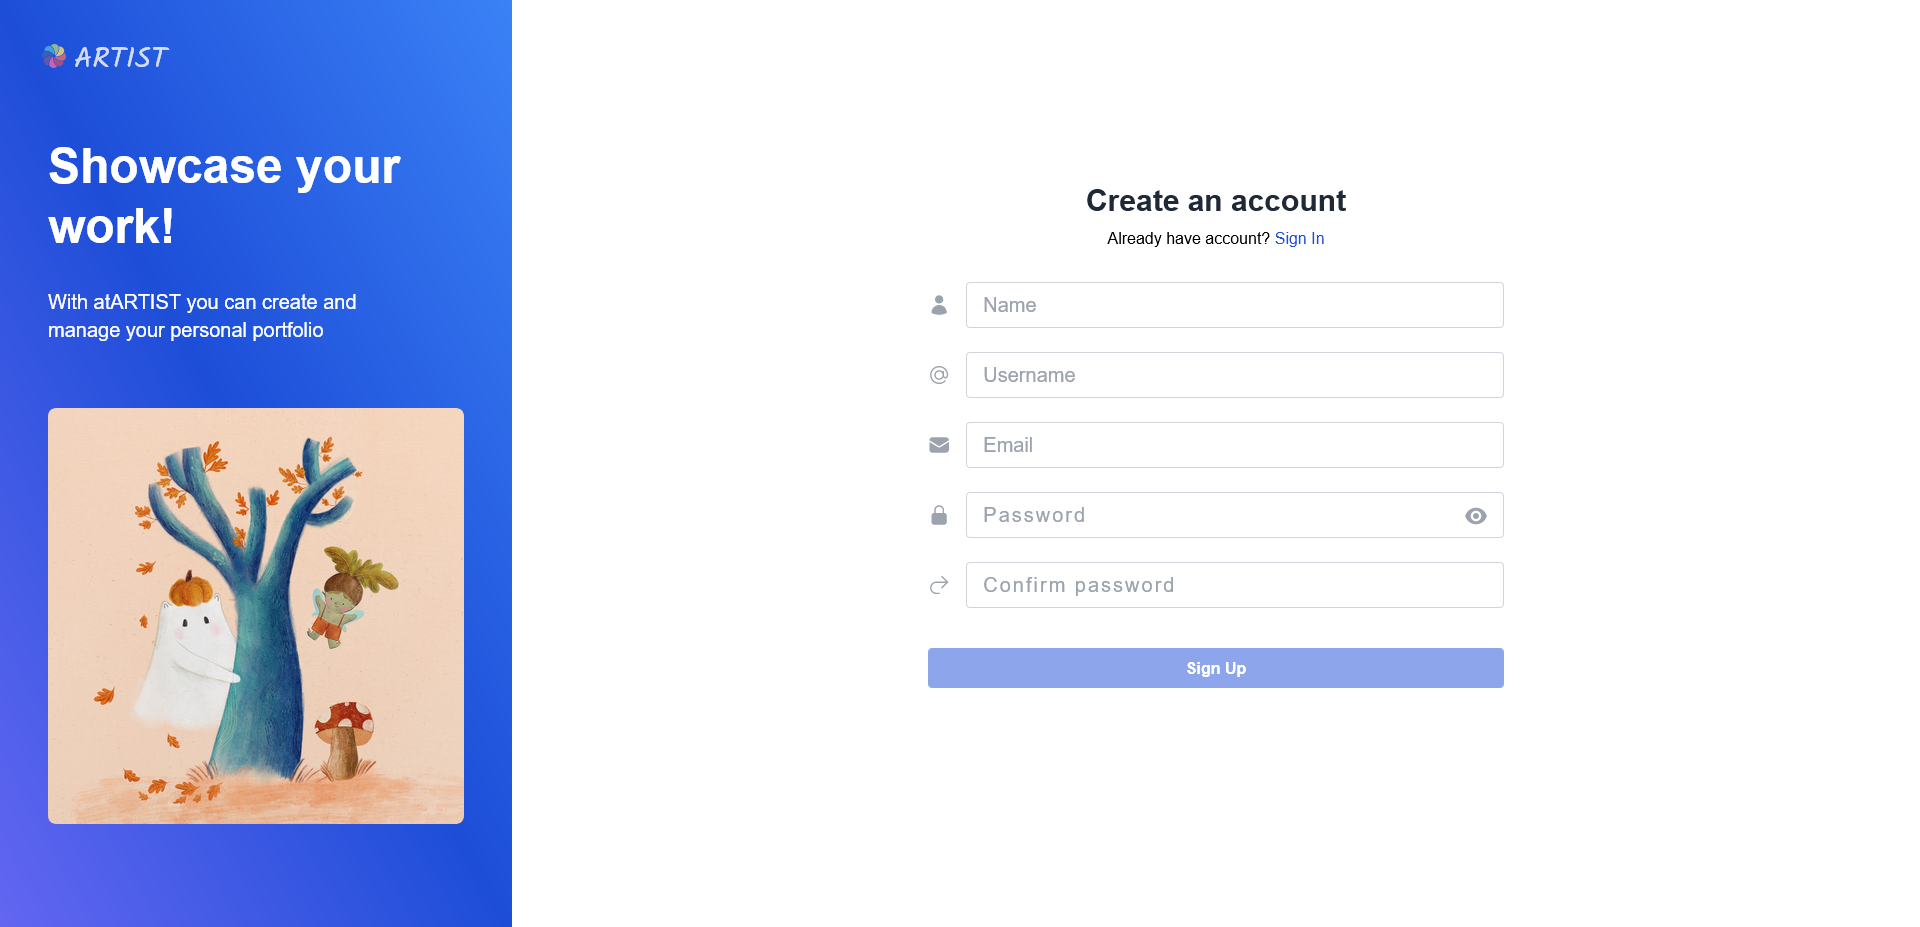
\includegraphics[width=1.0\linewidth]{figure/sign-up}}
	\caption{Pagina di registrazione}
	\label{fig:modulo_registrazione}
\end{figure}

Durante la compilazione del modulo viene verificata la disponibilit\`a dell'username, scelto dall'utente, attraverso la funzione \verb|availableUsername|, la quale invia una richiesta GET all'URI dell'API \verb|auth/username| passando l'username come parametro della richiesta. Se l'username non \`e disponibile viene mostrato un messaggio di errore al di sotto del campo ``username'' (Figura~\ref{fig:modulo_registrazione_non_valido}). In modo analogo viene verificata anche la disponibilit\`a dell'indirizzo e-mail attraverso la funzione \verb|availableEmail|.

Una volta che l'utente avr\`a compilato ogni campo, il modulo potr\`a essere inviato. Sar\`a quindi possibile eseguire la funzione \verb|signUp| la quale utilizza a sua volta l'azione \verb|signUp| dello store Pinia \verb|UserStore|. Tale azione invia i campi del modulo attraverso una richiesta POST all'URI dell'API \verb|auth/register|.

Se la richiesta ha successo verranno inizializzati gli stati \verb|user| e \verb|token| nello \verb|UserStore|. Inoltre, nella local storage del browser, verranno memorizzati l'access token, il valore \verb|expires_at| dell'acces token e il valore di \verb|remember_me|, impostato a \verb|true|.

Se la richiesta fallisce, vengono mostrati dei messaggi di errore al di sotto dei campi interessati in modo tale che l'utente possa correggerli (Figura~\ref{fig:modulo_registrazione_non_valido}).
\begin{figure}[htbp]
	\centering
	\fboxsep=0.5pt
	\fboxrule=0.5pt
	\fcolorbox{black}{black}{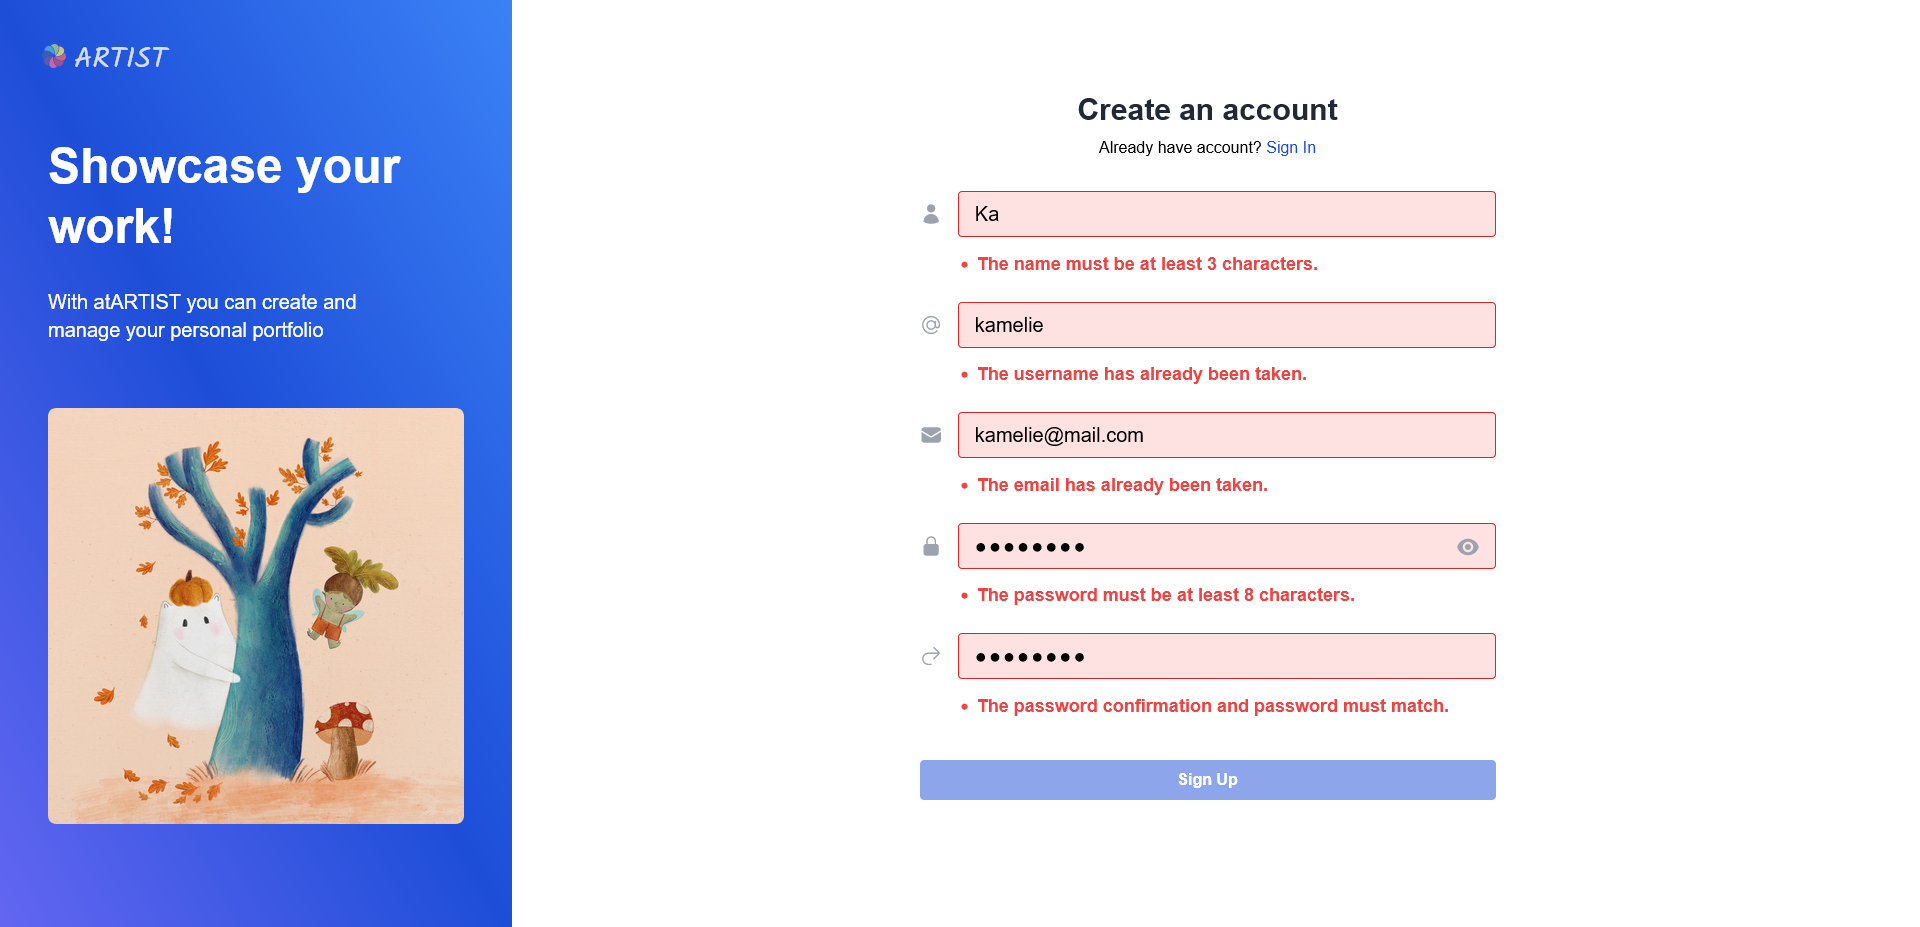
\includegraphics[width=1.0\linewidth]{figure/sign-up-error}}
	\caption{Pagina di registrazione con errori di validazione}
	\label{fig:modulo_registrazione_non_valido}
\end{figure}

Infine, una volta che il modulo \`e stato compilato ed elaborato correttamente, l'utente sar\`a autenticato e verr\`a reindirizzato alla homepage della piattaforma.

\subsection{Accesso}
\subsubsection{Laravel Route}
Per implementare l'accesso alla piattaforma \`e stata definita una sola route nel file \verb|routes/api/auth.php|  (Codice~\ref{lst:route_login}).
\\
\begin{lstlisting}[caption={Route per l'accesso}, label={lst:route_login}]
Route::post('login', [
	AuthenticatedTokenController::class, 'store'
]);
\end{lstlisting}
\subsubsection{AuthenticatedTokenController@store}
Il metodo \verb|store| della classe \verb|AuthenticatedTokenController| ha come unico parametro una richiesta di tipo \verb|AuthenticateRequest|. La classe \verb|AuthenticateRequest| si occupa di convalidare ogni richiesta, verificando che siano presenti i campi ``email'', ``password'' e ``remember\_me'', necessari per effettuare l'accesso, e che rispettino le regole definite nella classe \verb|Rules|.

Se la richiesta \`e valida viene eseguito il metodo, il quale:
\begin{itemize}
	\item Recupera l'utente dal valore della colonna ``email'' nella base di dati.
	\item Se l'utente viene trovato, la password con hash memorizzata nel database verr\`a confrontata con il valore della password nella richiesta attraverso il metodo \verb|check| della classe \verb|Hash|.
	\item Se le password sono diverse il metodo restituisce un messaggio di errore.
	\item Crea un token Sanctum.
	\item Se il campo \verb|remember_me| \`e falso verr\`a impostato l'attributo \verb|expires_at| del access token, con un valore pari alla data corrente pi\`u 24 ore.
\end{itemize} 

Se l'autenticazione ha avuto successo, il metodo restituisce come risposta il token per l'autenticazione e le informazioni dell'utente. In caso contrario, il metodo restituisce una risposta con codice di stato \verb|401| e contenente il messaggio \textit{``These credentials do not match our records''}.

\subsubsection{Pagina di accesso}
Per accedere alla piattaforma, l'utente si collega alla pagina ``auth/sign-in'' nella quale \`e presente il modulo di accesso. Tale modulo \`e rappresentato dal componente Vue \verb|AuthSignIn.vue|:

\begin{figure}[htbp]
	\centering
	\fboxsep=0.5pt
	\fboxrule=0.5pt
	\fcolorbox{black}{black}{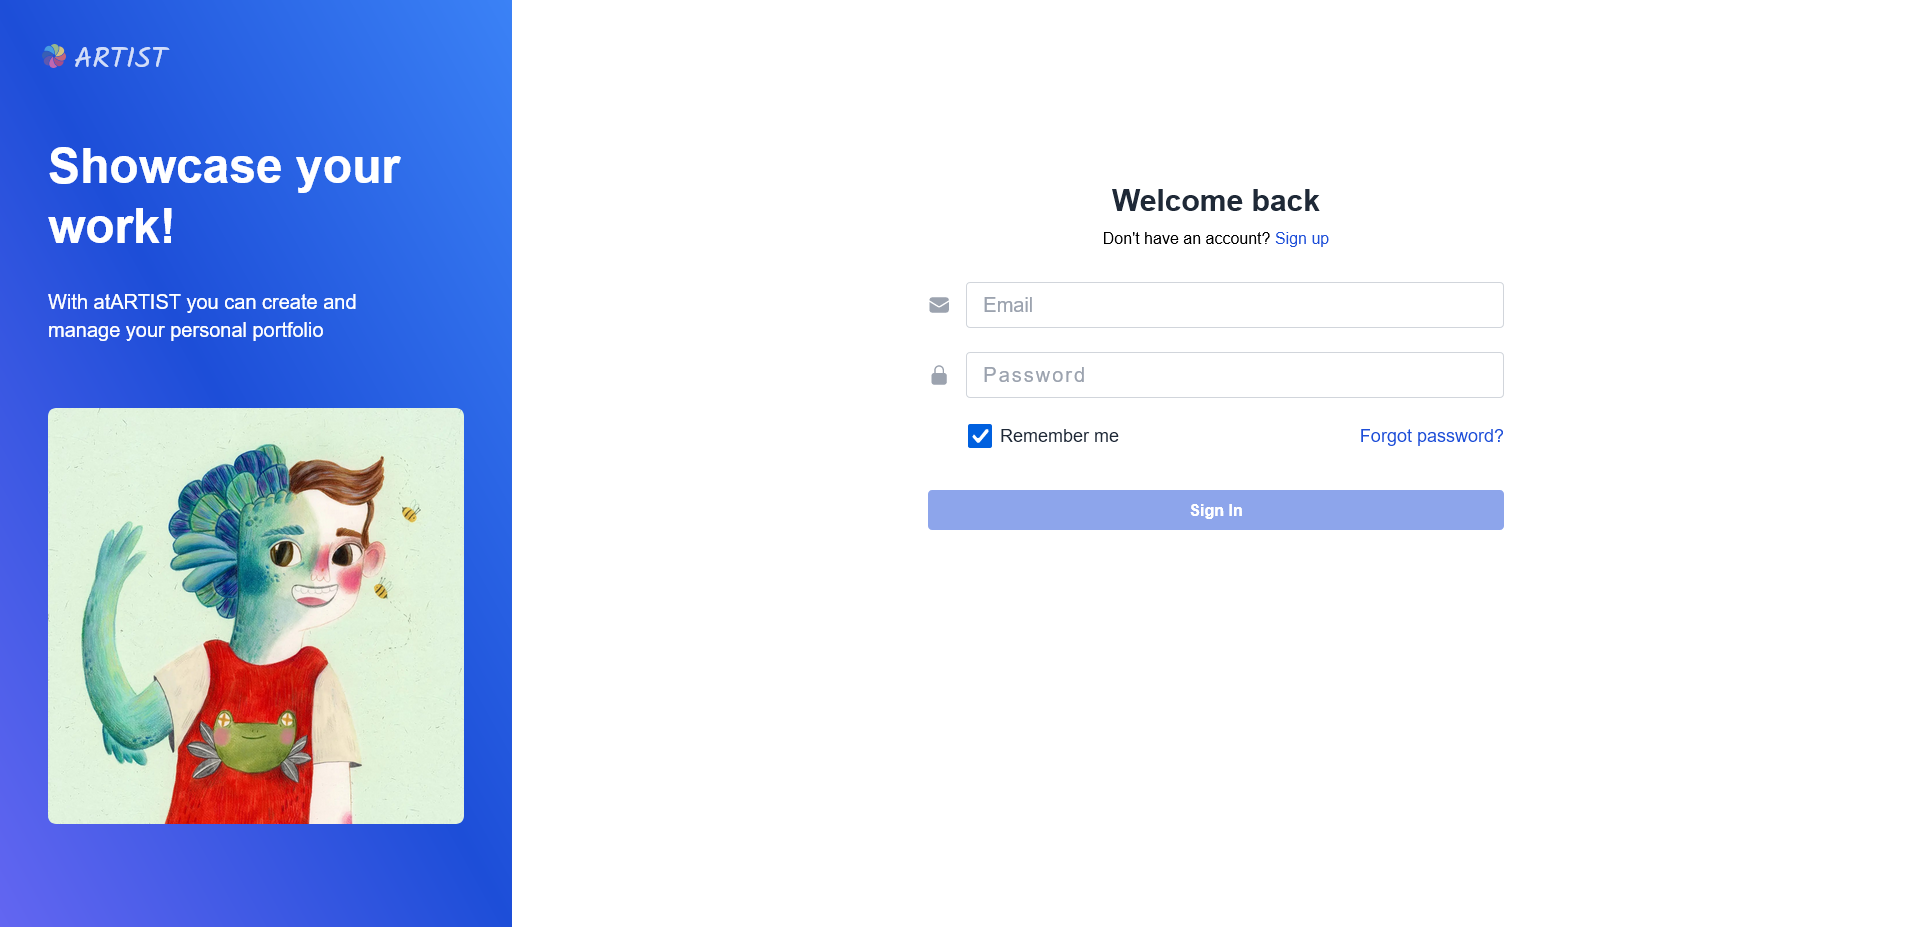
\includegraphics[width=1\linewidth]{figure/sign-in}}
	\caption{Pagina di accesso}
	\label{fig:sign_in_page}
\end{figure}

Una volta che l'utente avr\`a compilato ogni campo, il modulo potr\`a essere inviato. Sar\`a quindi possibile eseguire la funzione \verb|signIn| la quale utilizza a sua volta l'azione \verb|signIn| dello store Pinia \verb|UserStore|. Tale azione invia i campi del modulo attraverso una richiesta POST all'URI dell'API \verb|auth/login|.

Se la richiesta ha successo verranno inizializzati gli stati \verb|user| e \verb|token| nello \verb|UserStore|. Inoltre, nella local storage del browser, verranno memorizzati l'access token, il valore di \verb|remember_me| e  il valore \verb|expires_at| dell'access token.

Se la richiesta fallisce, a causa di errori di validazione, vengono mostrati dei messaggi di errori al di sotto dei campi interessati in modo tale che l'utente possa correggerli. Nel caso in cui credenziali d'accesso fornite non corrispondano con quelle memorizzate nel database, viene mostrato un messaggio di errore in cima al modulo (Figura~\ref{fig:sign_in_page_error}).
\begin{figure}[htbp]
	\centering
	\fboxsep=0.5pt
	\fboxrule=0.5pt
	\fcolorbox{black}{black}{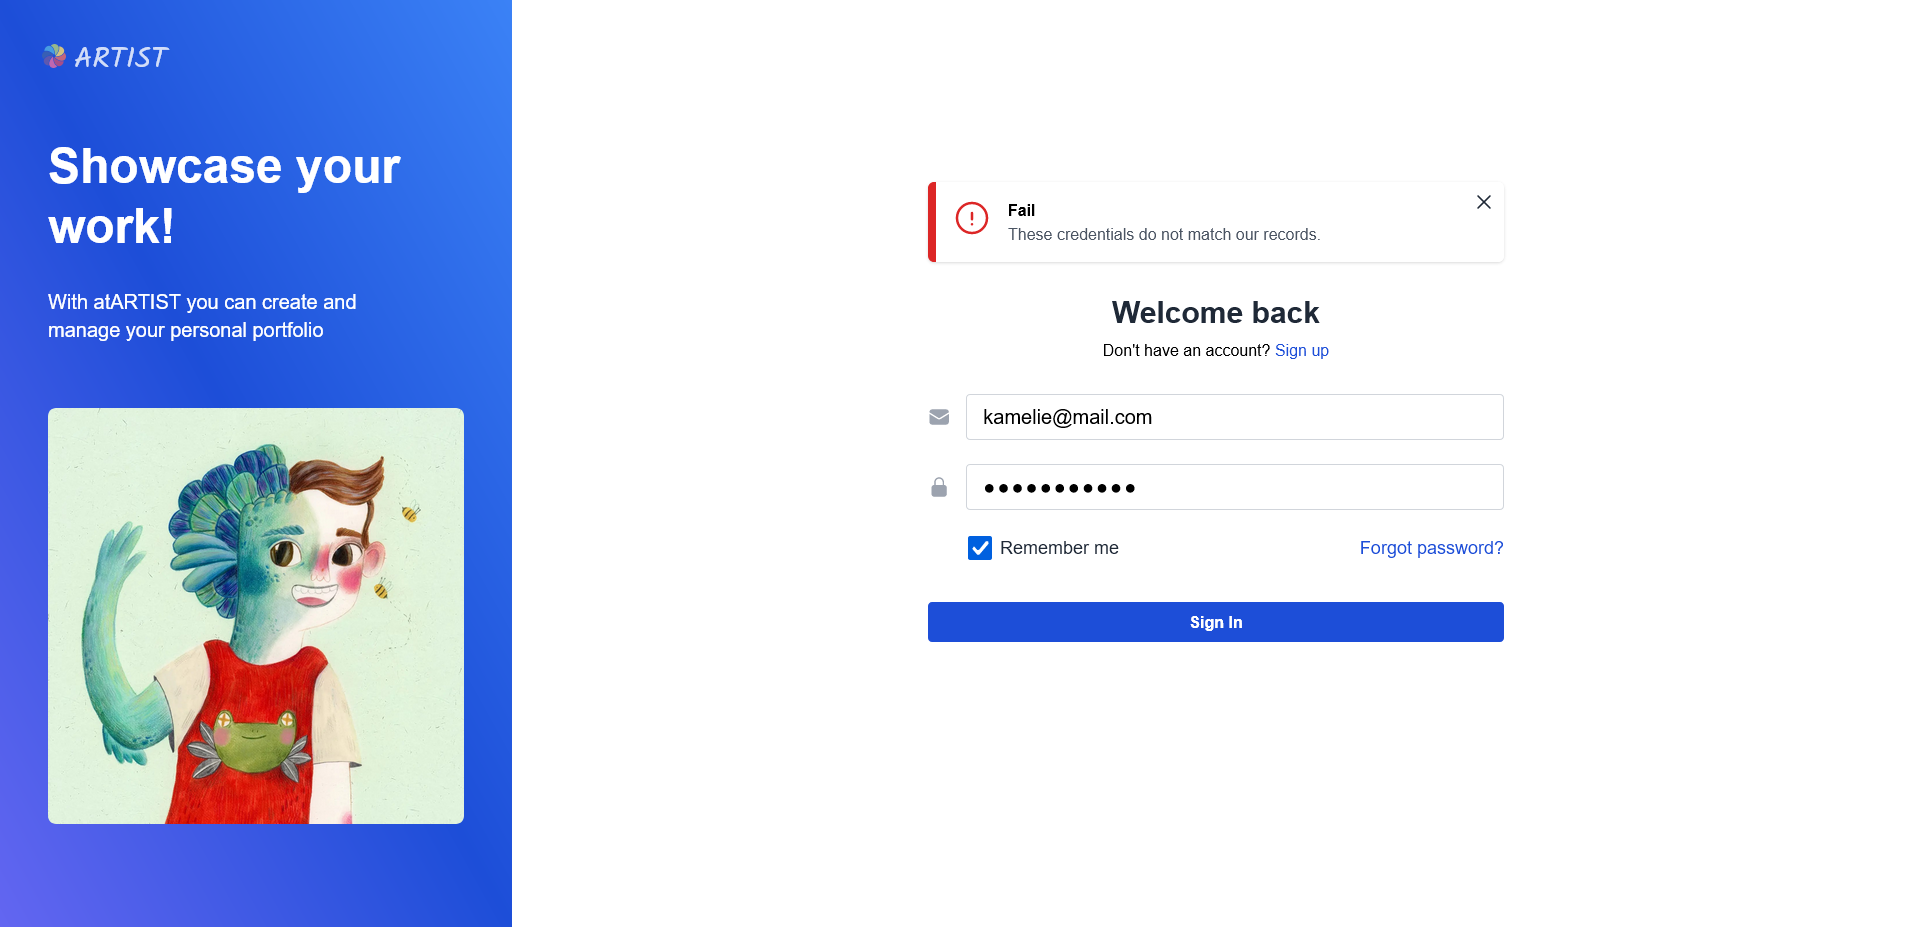
\includegraphics[width=1\linewidth]{figure/sign-in-error}}
	\caption{Pagina di accesso con credenziali errate}
	\label{fig:sign_in_page_error}
\end{figure}

Infine, una volta che il modulo \`e stato compilato ed elaborato correttamente, l'utente sar\`a autenticato e verr\`a reindirizzato alla homepage della piattaforma.
\subsection{Disconnessione}
\subsubsection{Laravel Route}
Per implementare la disconnessione dalla piattaforma \`e stata definita una sola route nel file \verb|routes\api\auth.php|:
\begin{lstlisting}[caption={Route per la disconnessione}, label={lst:route_logout}]
Route::delete('logout', [
	AuthenticatedTokenController::class, 'destroy'
])->middleware('auth:api');
\end{lstlisting}

\subsubsection{AuthenticatedTokenController@destroy}
Il metodo \verb|destroy| della classe \verb|AuthenticatedTokenController| non ha parametri. Tale metodo si occupa di eliminare l'access token con il quale \`e stata eseguita la richiesta e restituisce il messaggio \textit{``User logged out''}.

\subsubsection{Disconnessine dalla piattaforma}
Per effettuare la disconnessione dalla piattaforma, l'utente preme il pulsante ``Sign out'' presente nel men\`u a tendina nella barra di navigazione della piattaforma (Figura~\ref{fig:nav-bar-auth}). Tale pulsante esegue la funzione \verb|signOut| la quale utilizza a sua volta l'azione \verb|signOut| dello store Pinia \verb|UserStore|. Tale azione effettua una richiesta DELETE all'URI dell'API \verb|auth/logout| e se essa ha successo vengono rimossi dalla local storage i valori \verb|user_token|,  \verb|remember_me| e \verb|session_expires_at|.

Infine, l'utente verr\`a portato alla homepage della piattaforma effettuando un refresh della pagina in modo tale da resettare lo stato dell'applicazione.

\section{Gestione utente}
La gestione dell'utente consiste, principalmente, nella realizzazione delle componenti necessarie per ottenere le informazioni dell'utente autenticato alla piattaforma e delle componenti per la eliminazione e ripristino del suo account.

\subsection{Utente autenticato}
\subsubsection{Laravel Route}
Per ottenere le informazioni dell'utente autenticato alla piattaforma \`e stata definita una sola route nel file \verb|routes\api\auth.php|:
\begin{lstlisting}[caption={Route per ottenere l'utente autenticato}, label={lst:route_logout}]
Route::get('user', [AuthenticatedTokenController::class, 'show']);
\end{lstlisting}

\subsubsection{AuthenticatedTokenController@show}
Il metodo \verb|show| della classe \verb|AuthenticatedTokenController| ha come unico paramento una normale richiesta. Non \`e protetto da nessun middleware, la verifica del access token avviene all'interno del metodo per permettere di ottenere le informazioni dell'utente anche quando questo viene eliminato.

La validit\`a del access token viene verificata utilizzando il metodo \verb|findToken| della classe \verb|Laravel\Sanctum\PersonalAccessToken|.

Se l'access token non \`e valido il metodo viene interrotto da una \verb|UnauthorizedHttpException| che restituir\`a una risposta con codice di stato \verb|403| e contenente il messaggio \textit{``Access denied''}.

Tramite l'access token \`e possibile recuperare l'utente dalla base di dati, il quale viene restituito come risposta.

\subsubsection{Layout principale}
Il layout principale delle sezioni della piattaforma \`e rappresentato dal componente Vue \verb|DefaultLayout.vue| ed \`e composto dalla barra di navigazione  della piattaforma, rappresentata dal componente Vue \verb|NavBar.vue|, e da una \verb|RouterView| nella quale verr\`a montato il contenuto della pagina.

Quando un utente si collega alla piattaforma, nel layout principale  viene eseguita l'azione \verb|setToken| dello store Pinia \verb|UserStore|, la quale verifica se:
\begin{itemize}
	\item Il valore \verb|user_token| \`e presente nella local storage.
	\item Il valore \verb|remember_me| \`e vero e in tal caso restituisce l'access token.
	\item L'accesso token \`e ancora valido confrontando la data e ora attuale con quella di scadenza del token e in tal caso lo restituisce. Se il token \`e scaduto, rimuove le informazioni riguardo la sessione dalla local storage.
\end{itemize}

Se l'utente non ha un access token, nella barra di navigazione saranno presenti i link per registrarsi e per accedere alla piattaforma (Figura~\ref{fig:nav-bar-guest}). Se, invece, l'utente \`e autenticato, nella barra di navigazione sar\`a presente la sua foto di profilo che gli permetter\`a di espandere un men\`u a tendina nel quale sono presenti i suoi dati e le sezioni della piattaforma che richiedono l'autenticazione (Figura~\ref{fig:nav-bar-auth}).

\begin{figure}[htbp]
	\centering
	\fboxsep=0.5pt
	\fboxrule=0.5pt
	\fcolorbox{black}{black}{
\includegraphics[width=1.0\linewidth]{figure/nav-bar-guest}}
	\caption{Barra di navigazione per l'utente ospite}
	\label{fig:nav-bar-guest}
\end{figure}

\begin{figure}[htbp]
	\centering
	\fboxsep=0.5pt
	\fboxrule=0.5pt
	\fcolorbox{black}{black}{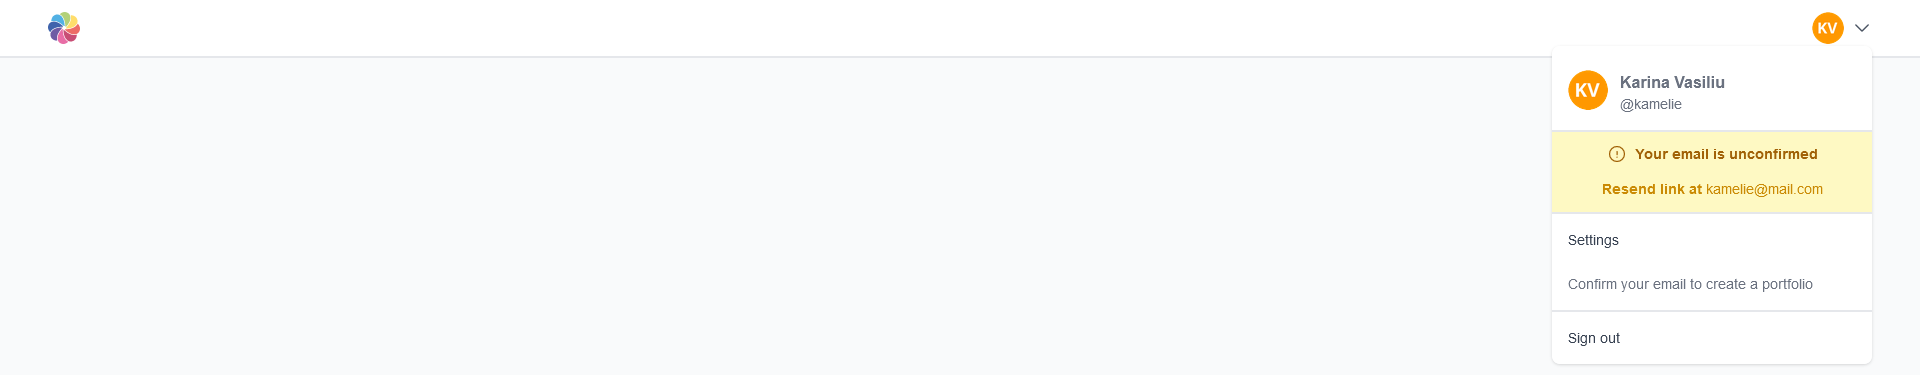
\includegraphics[width=1.0\linewidth]{figure/nav-bar-auth}}
	\caption{Barra di navigazione per l'utente autenticato}
	\label{fig:nav-bar-auth}
\end{figure}

\subsection{Eliminazione e ripristino account}

\subsubsection{Laravel Route}
Per implementare l'eliminazione ed il ripristino dell'account sono state definite due route nel file \verb|routes\api\v1\api.php|:
\begin{lstlisting}[caption={Route per l'eliminazione e ripristino dell'account}, label={lst:route_user_delete}]
Route::delete('users/{user}',  [UserController::class, 'destroy'])
	->middleware(['auth:api', 'ability:password.confirm']);
Route::patch('users/{user}/delete', [
	UserDeleteController::class, 'update'
]);
\end{lstlisting}
Inoltre, per effettuare l'eliminazione, \`e necessario che l'utente confermarmi nuovamente la password, a tal fine \`e stata definita la route nel file \verb|routes\api\v1\auth.php| (Codice~\ref{lst:route_confirm_psw}).
\begin{lstlisting}[caption={Route per la conferma della password}, label={lst:route_confirm_psw}]
Route::post('confirm-password', [
	ConfirmablePasswordController::class, 'store'
])->middleware(['auth:api', 'throttle:6,1']);
\end{lstlisting}

\subsubsection{ConfirmablePasswordController@store}
Il metodo \verb|store| della classe \verb|ConfirmablePasswordController| ha come unico parametro una richiesta di tipo \verb|ConfirmablePasswordRequest|. La classe \verb|ConfirmablePasswordRequest| si occupa di convalidare ogni richiesta, verificando che sia presente il campo ``password'', necessario per effettuare la verifica della password e che rispetti le regole definite nella classe \verb|Rules|.

Se la richiesta \`e valida viene eseguito il metodo, il quale:
\begin{itemize}
	\item Confrontata la password con hash, memorizzata nel database, dell'utente autenticato con il valore della password nella richiesta attraverso il metodo \verb|check| della classe \verb|Hash|.
	\item Crea un token Sanctum dotato dell'abilit\`a \verb|password.confirm| con validit\`a di un'ora.
\end{itemize} 

Il metodo restituisce come risposta il token per la conferma della password.

\subsubsection{UserController@destroy}
Il metodo \verb|destroy| della classe \verb|UserController| ha come unico parametro l'utente. Tale metodo \`e protetto dal middleware \verb|ability:password.confirm| per verificare che l'utente abbia confermato la password prima di eseguire la richiesta.

Il metodo elimina prima tutti gli access token creati dall'utente e poi l'utente. Infine, restituisce come risposta il messaggio \textit{``User deleted successfully''}.

\subsubsection{UserDeleteController@update}
Il metodo \verb|update| della classe \verb|UserDeleteController| ha come parametri una normale richiesta e lo username. Non \`e protetta da nessun middleware, la verifica del access token avviene all'interno del metodo in quanto i meccanismi di Sanctum ignorano i modelli eliminati. 

Come prima cosa, il metodo recupera l'utente eliminato dal valore della colonna ``username''. Se l'utente trovato non \`e stato eliminato, il metodo  viene interrotto da una
\verb|HttpResponseException| che restituir\`a una risposta con codice di stato \verb|404| e contenente il messaggio \textit{``This user isn't deleted''}.

Successivamente, si verifica la validit\`a del access token utilizzando il metodo \verb|findToken| della classe \verb|Laravel\Sanctum\PersonalAccessToken|. Se l'access token non \`e valido il metodo viene interrotto da una \verb|UnauthorizedHttpException| che restituir\`a una risposta con codice di stato \verb|403| e contenente il messaggio \textit{``Access denied''}.

Tramite il token \`e possibile risalire all'utente che ha effettualo la richiesta e verificare, quindi, se sia lo stesso utente recuperato dal database precedentemente.
In tal caso, l'utente viene ripristinato.

Il metodo restituisce come risposta il messaggio \textit{``User restored successfully''}.

\subsubsection{Eliminazione definitiva}
Gli utenti che non eseguono il ripristino del proprio account entro 60 giorni verranno automaticamente eliminati. Per far ci\`o \`e presente un'utilit\`a di pianificazione nel metodo \verb|schedule| della classe \verb|App\Console\Kernel|:

\begin{lstlisting}[caption={Utilit\`a di pianificazione per l'eliminazione definitiva degli utenti}, label={lst:user_hard_delete}]
$schedule->call(function () {
	$users = User::onlyTrashed()->where(
		'deleted_at',
		'<=',
		now()->subDays(60)->toDateTimeString()
	)->get();
	
	$users->each->forceDelete();
})->daily();
\end{lstlisting}

\subsubsection{Pagina eliminazione account}
Tramite la voce ``Delete account'' del men\`u delle impostazioni \`e possibile collegarsi alla pagina ``settings/delete-account'' per l'eliminazione del proprio account. Tale pagina \`e rappresentata dal componente Vue \verb|UserSettingsDeleteAccount.vue| (Figura~\ref{fig:user_settings_delete_account}) ed \`e composta da un modulo per fornire nuovamente la password.

\begin{figure}[htbp]
	\centering
	\fboxsep=0.5pt
	\fboxrule=0.5pt
	\fcolorbox{black}{black}{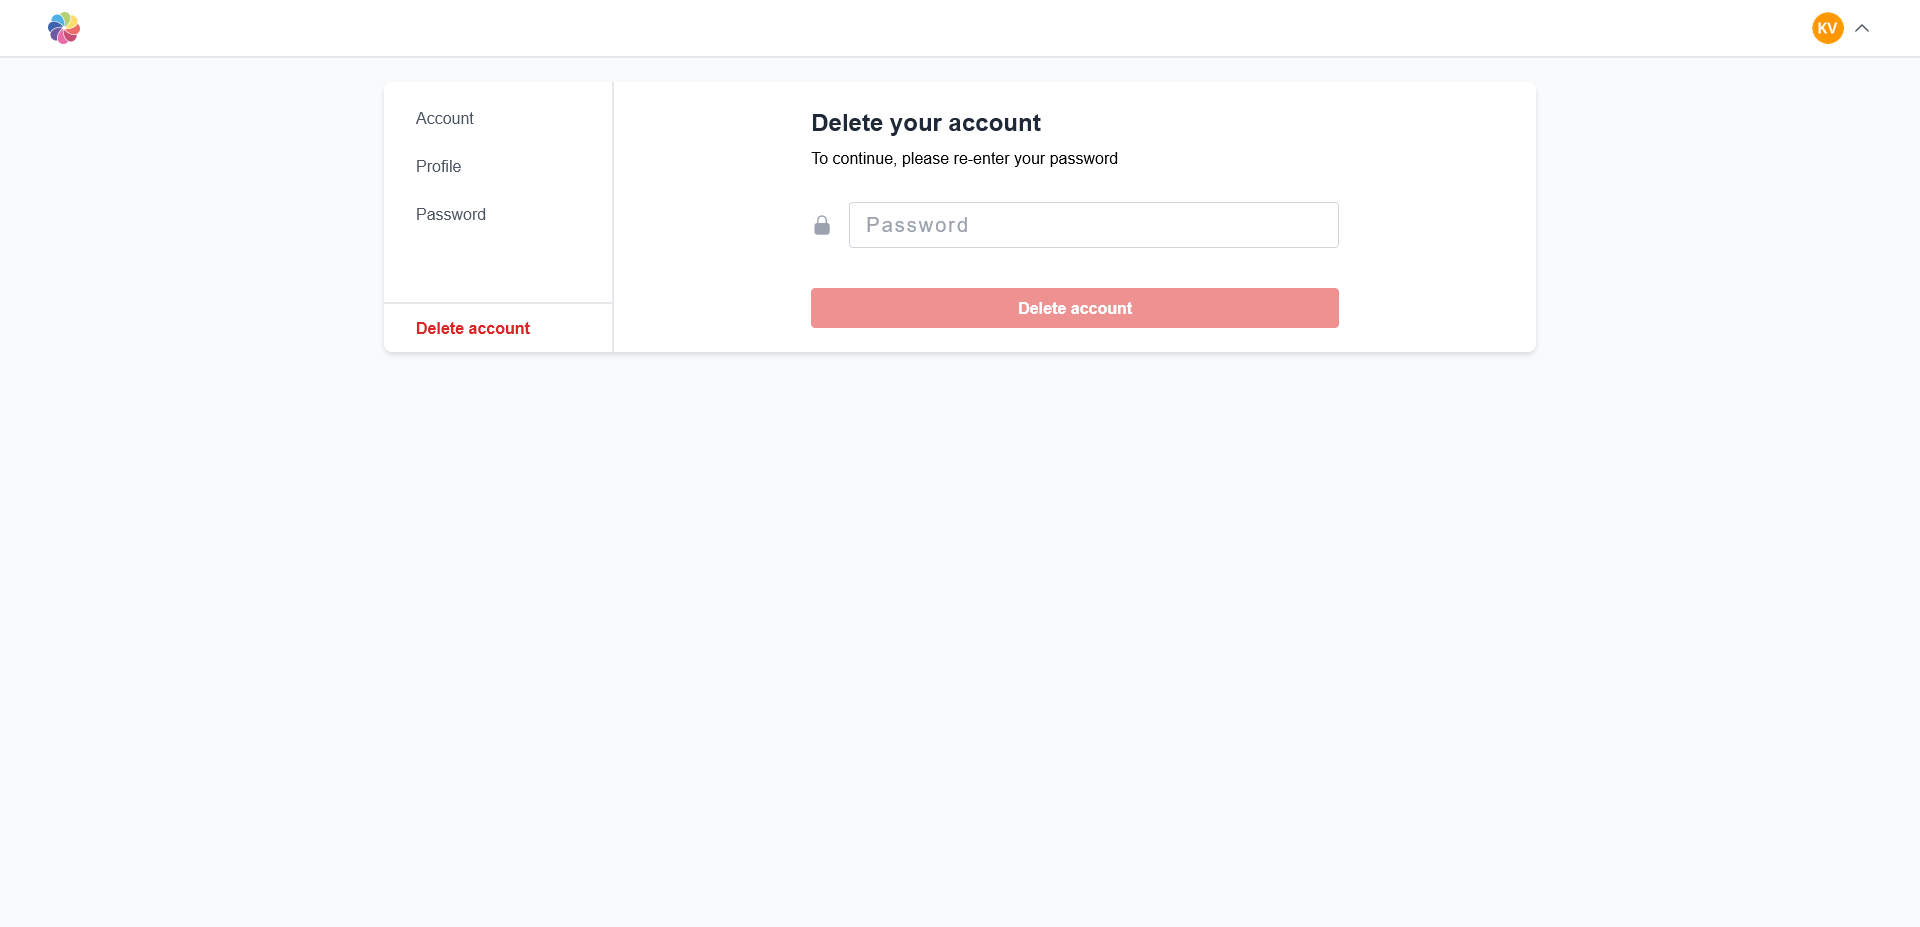
\includegraphics[width=1.0\linewidth]{figure/delete_account}}
	\caption{Pagina eliminazione account}
	\label{fig:user_settings_delete_account}
\end{figure}

Una volta che l'utente ha compilato il campo ``password'' il modulo potr\`a essere inviato. Sar\`a quindi possibile eseguire la funzione \verb|deleteAccount| la quale, innanzitutto, invia il campo ``password'' attraverso una richiesta POST all'URI dell'API \verb|auth/confirm-password|. Se la password fornita non corrisponde con quella memorizzata nel database viene mostrato un messaggio di errore in cima al modulo. 

Se la richiesta ha successo restituisce un access token con il quale \`e possibile effettuare una richiesta DELETE all'URI dell'API \verb|v1/users/{user}|. 

Infine, una volta che anche la seconda richiesta \`e stata elaborata correttamente, verranno rimosse le informazioni riguardo la sessione dalla local storage del browser e l'utente verr\`a reindirizzato alla homepage della piattaforma.

\subsubsection{Pagina ripristino dell'account}
Tramite l'attributo \verb|active| dello stato \verb|user|, presente nello store Pinia \verb|UserStore| a seguito dell'autenticazione dell'utente, \`e possibile verificare se l'utente ha eliminato il proprio account. In tale caso, l'utente verr\`a portato alla pagina ``auth/restore-account'' per ripristinare il proprio account.

La pagina di ripristino account \`e rappresentata dal componente Vue \verb|RestoreAccountView.vue| la quale \`e composta da un pulsante per il ripristino dell'account.


Se l'utente decide di ripristinare l'account, premendo il pulsante ``Restore'', viene eseguito la funzione \verb|restoreAccount| la quale utilizza a sua volta l'azione \verb|restoreAccount| dello store. Tale azione effettua una richiesta PATCH all'URI dell'API \verb| v1/users/{user}/delete|.

Infine, una volta che la richiesta \`e stata elaborata correttamente, il valore \verb|active| viene impostato a \verb|true| e l'utente viene reindirizzato alla homepage della piattaforma.

\section{Gestione del portfolio}
La gestione dell'portfolio consiste, principalmente, nella realizzazione delle componenti necessarie per la creazione di un nuovo portfolio e per la visualizzazione delle sue sezioni pubbliche.

\subsection{Operazioni principali}
\subsubsection{Laravel Route}
Per implementare le operazioni principali sul portfolio sono state definite, attraverso il metodo \verb|apiResource| della classe \verb|Route|, le route per l'utilizzo dei metodi \verb|store|, \verb|show|, \verb|update| e \verb|destroy| della classe \verb|CMS\Portfolio\PortfolioController| nel file \verb|routes\api\v1\cms.php|:
\begin{lstlisting}[caption={Route per le operazioni principali sul portfolio}, label={lst:route_logout}]
Route::apiResource('portfolios', PortfolioController::class)
	->except(['index']);
\end{lstlisting}

\subsubsection{PortfolioController@store}
Il metodo \verb|store| della classe \verb|PortfolioController| ha come unico parametro una richiesta di tipo \verb|CreatePortfolioRequest|. La classe \verb|CreatePortfolioRequest| si occupa di convalidare ogni richiesta, verificando che sia presente il campo ``name'', necessario per effettuare la creazione del portfolio e che rispetti le regole definite nella classe \verb|PortfolioRules|. 

Se la richiesta \`e valida viene eseguito il metodo, il quale:
\begin{itemize}
	\item Crea un nuovo portfolio nella base di dati.
	\item Crea, nella base di dati, la sezione ``home'' del portfolio e la sua relativa galleria.
	\item Crea, nella base di dati, la sezione ``about-me'' del portfolio e la sua relativa biografia e contatto.
\end{itemize} 

Il metodo restituisce come risposta le informazioni del portfolio e delle sue sezioni, secondo quanto specificato nella classe \verb|NewPortfolioResource|: 
	
\begin{lstlisting}[caption={Risposta di successo creazione del portfolio}, label={lst:response_success_portfolio}, tabsize=3]
{
	"status": "success",
	"data": {
		"message": "Portfolio created successfully",
		"portfolio": {
			"name": "kamelie",
			"icon": "media/portfolio/icon/default.png",
			"active": true,
			"archived": false,
			"galleries_count": 1,
			"sections": {
				"galleries": [
					{
						"category": "gallery",
						"slug": "home",
						"name": "Home",
						"posts_count": 0,
						"index": 1,
						"description": "Welcome to kamelie's
										Portfolio!",
						"archived": false
					}
				],
				"about_me": {
					"category": "about-me",
					"name": "About me",
					"slug": "about-me",
					"archived": false
				}
			}
		}
	}
}
\end{lstlisting}

\subsubsection{Pagina di creazione del portfolio}
Un utente, che abbia verificato il proprio indirizzo e-mail, pu\`o collegarsi alla pagina principale della sezione CMS della piattaforma tramite la voce ``Manage your portfolio'' del men\`u a tendina nella barra di navigazione. Se l'utente che non ha ancora creato un proprio portfolio viene reindirizzato alla pagina ``portfolio/new'' nella quale \`e presente il modulo di creazione del portfolio. Tale modulo \`e rappresentato dal componente Vue \verb|PortfolioCreate.vue| (Figura~\ref{fig:pagina_creazione_portfolio}). 

\begin{figure}[htbp]
	\centering
	\fboxsep=0.5pt
	\fboxrule=0.5pt
	\fcolorbox{black}{black}{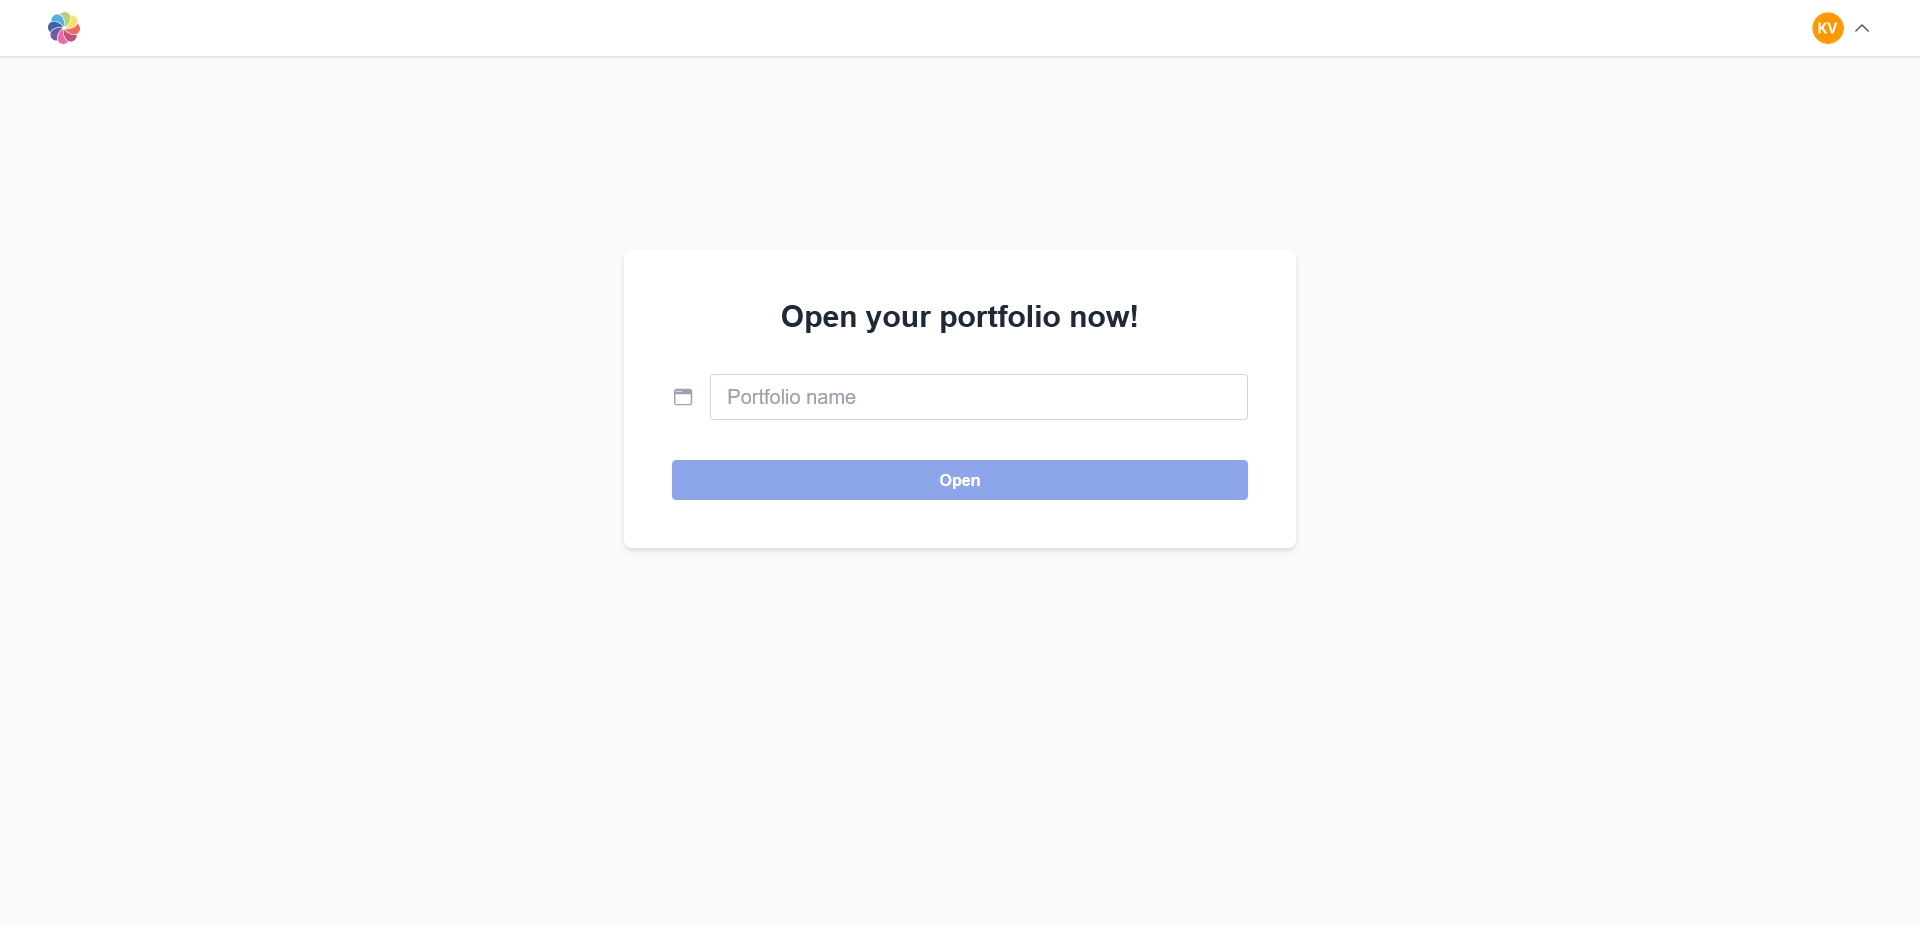
\includegraphics[width=1.0\linewidth]{figure/portfolio-new}}
	\caption{Pagina di creazione del portfolio}
	\label{fig:pagina_creazione_portfolio}
\end{figure}

Una volta che l'utente avr\`a compilato il campo ``name'', il modulo potr\`a essere inviato. Sar\`a quindi possibile eseguire la funzione \verb|createPortofolio| la quale utilizza a sua volta l'azione \verb|createPortofolio| dello store Pinia \verb|CMSStore|. Tale azione invia il campo del modulo attraverso una richiesta POST all'URI dell'API \verb|v1/cms/portfolios| e se essa ha successo verranno inizializzati gli stati \verb|portfolio|, che conterr\`a le informazioni sul portfolio, e \verb|galleries|, che conterr\`a la lista di gallerie, nello \verb|CMSStore|.

Infine, una volta che il modulo \`e stato compilato ed elaborato correttamente, l'utente verr\`a reindirizzato alla pagina principale della sezione CMS della piattaforma.

\subsection{Visualizzazione del portfolio utente}
Per ottenere le informazioni sul portfolio dell'utente autenticato alla piattaforma \`e stata definita una sola route nel file \verb|routes\api\v1\cms.php|:
\begin{lstlisting}[caption={Route per ottenere il portfolio dell'utente autenticato}, label={lst:route_logout}]
Route::get('/', [CMSController::class, 'show']);
\end{lstlisting}

\subsubsection{CMSController@show}
Il metodo \verb|show| della classe \verb|CMSController| ha come unico paramento una normale richiesta. Tale metodo si occupa di ottenere il portfolio dell'utente autenticato utilizzando il metodo \verb|portfolio| del modello \verb|User|, il quale restituisce la relazione tra utente e portfolio. Tale relazione considera anche il caso in cui il portfolio sia stato eliminato, in modo tale che sia possibile ottenere comunque le sue informazioni.


Il metodo restituisce le informazioni del portfolio trovato, secondo quanto specificato nella classe \verb|PortfolioInfoResource| (Codice~\ref{lst:response_success_portfolio_info}).

Se l'utente non ha nessun portfolio associato, il metodo viene interrotto e restituisce una risposta con codice di stato \verb|404|.

\begin{lstlisting}[caption={Risposta di successo visualizzazione del portfolio utente}, label={lst:response_success_portfolio_info}]
{
	"status": "success",
	"data": {
		"portfolio": {
			"name": "kamelie",
			"icon": "media/portfolio/icon/icon-1.png",
			"active": true,
			"archived": false,
			"galleries_count": 3
		}
	}
}
\end{lstlisting}

\subsubsection{Layout CMS}
Il layout per la sezione CMS della della piattaforma \`e rappresentato dal componente Vue \verb|LayoutCMSLayout.vue| ed \`e composto dalla barra laterale di navigazione delle sezioni dedicate alla gestione dei contenuti del portfolio, rappresentata dal componente Vue \verb|SideBar.vue|, e da una \verb|RouterView| nella quale verr\`a montato il contenuto della pagina.

Quando un utente si collega ad una sezione del CMS, viene eseguita l'azione \verb|getPortfolio| dello store Pinia \verb|CMSStore|, la quale restituisce lo stato \verb|portfolio|. Se lo stato non ha attributi viene eseguita l'azione \verb|fetchPortfolio| che effettua una richiesta GET all'URI dell'API \verb|v1/cms| per ottenere le informazioni sul portfolio utente .

Se la richiesta ha successo verr\`a inizializzato lo stato \verb|portfolio|. Se, invece, la richiesta fallisce l'utente viene reindirizzato alla pagina di creazione del portfolio (Figura~\ref{fig:pagina_creazione_portfolio}).

Infine, se la richiesta ha successo ma l'attibuto \verb|active| \`e \verb|false| l'utente viene reindirizzato alla pagina ``portfolio/restore'' per il ripristino e l'eliminazione definitiva del portfolio.


\subsubsection{Pagina principale della sezione CMS}
Per gestire il proprio portfolio l'utente si collega alla pagina ``portfolio'' rappresentata dal componente Vue \verb|CMSHome.vue| (Figura~\ref{fig:cms-home}).
\begin{figure}[htbp]
	\centering
	\fboxsep=0.5pt
	\fboxrule=0.5pt
	\fcolorbox{black}{black}{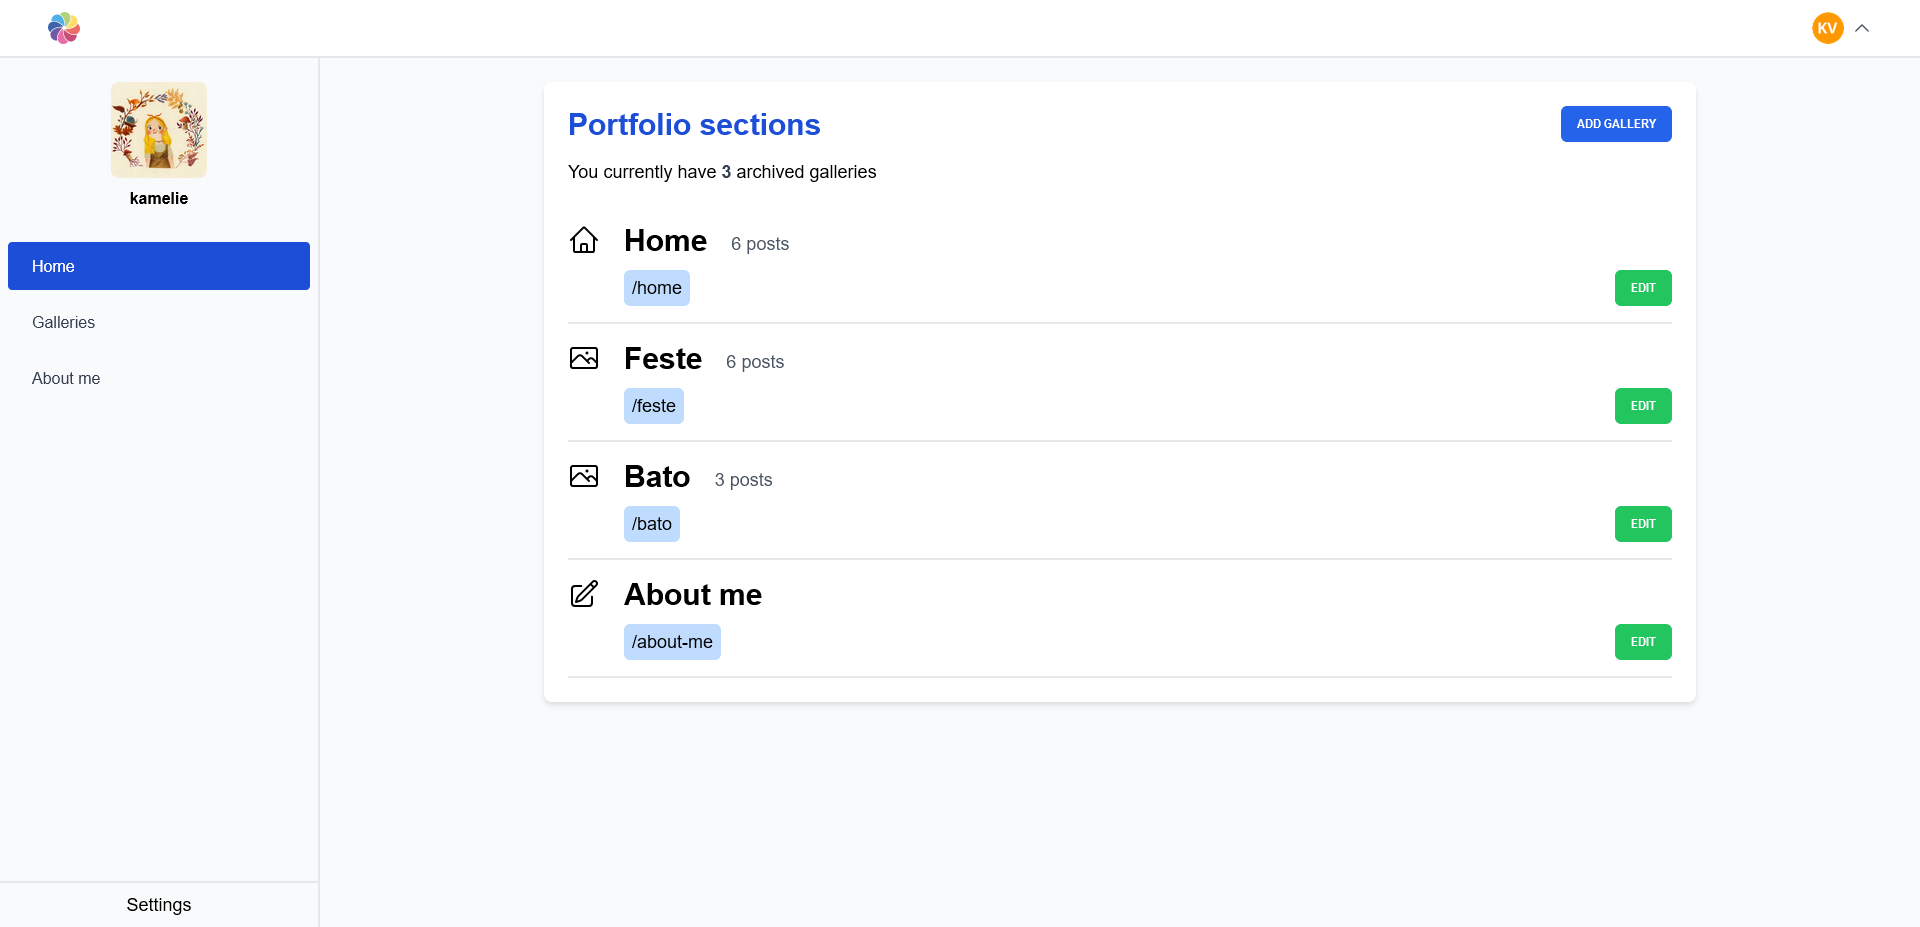
\includegraphics[width=1.0\linewidth]{figure/cms-home}}
	\caption{Pagina principale della sezione CMS}
	\label{fig:cms-home}
\end{figure}

Durante il caricamento della pagina, viene eseguita l'azione \verb|getGalleries| dello store Pinia \verb|CMSStore|, la quale restituisce lo stato \verb|galleries|. Se tale stato non ha attributi viene eseguita l'azione \verb|fetchGalleries| che effettua una richiesta GET all'URI dell'API \verb|v1/cms/portfolios/{portfolio}/galleries| per ottenere le gallerie del portfolio utente. Se la richiesta ha successo verr\`a inizializzato lo stato \verb|galleries|. 

Infine, le gallerie presenti nello stato vengono filtrate, in modo tale da visualizzare solo quelle non archiviate, utilizzando l'attributo \verb|archived|.

\section{Gestione delle gallerie}
La gestione delle gallerie consiste nella realizzazione delle componenti necessarie per creare, visualizzare, modificare, archiviare, eliminare e ripristinare le gallerie e nella realizzazione delle componenti necessarie per gestire i post della galleria. 

\subsection{Operazioni principali}
\subsubsection{Laravel Route}
Per implementare le operazioni principali sulle gallerie sono state definite, attraverso il metodo \verb|apiResource| della classe \verb|Route|, le route per l'utilizzo dei metodi \verb|index|, \verb|store|, \verb|show|, \verb|update| e \verb|destroy| della classe \verb|CMS\Gallery\GalleryController| nel file \verb|routes\api\v1\cms.php|:
\begin{lstlisting}[caption={Route operazioni principali sulle gallerie}, label={lst:route_g_crud}]
Route::apiResource(
	'portfolios.galleries',
	GalleryController::class
);
\end{lstlisting}

\subsubsection{GalleryController@index}
Il metodo \verb|index| della classe \verb|GalleryController| ha come unico parametro il portfolio e restituisce le informazioni delle gallerie, non eliminate, del portfolio, le quali vengono specificate nella classe \verb|GalleriesResource| (Codice~\ref{lst:response_success_gallery_list}).
\begin{lstlisting}[caption={Risposta di successo lista delle gallerie}, label={lst:response_success_gallery_list}]
{
	"status": "success",
	"data": {
		"galleries": [
			{
				"category": "gallery",
				"slug": "home",
				"name": "Home",
				"posts_count": 6,
				"index": 1,
				"description": "I mei ultimi lavori",
				"archived": false
			},
			...
		]
	}
}
\end{lstlisting}


\subsubsection{GalleryController@store}
Il metodo \verb|store| della classe \verb|GalleryController| ha come parametri una richiesta di tipo \verb|CreateGalleryRequest| e il portfolio. La classe \verb|CreateGalleryRequest| si occupa di convalidare ogni richiesta, verificando che siano presenti i campi ``name'' e ``description'', necessari per effettuare la creazione della galleria e che rispettino le regole definite nelle classi \verb|GalleryRules| e \verb|SectionRules|. 

Se la richiesta \`e valida viene eseguito il metodo, il quale:
\begin{itemize}
	\item Crea una nuova sezione nella base di dati.
	\item Crea una nuova galleria nella base di dati.
\end{itemize} 

Il metodo restituisce come risposta le informazioni sulla galleria creata e il messaggio \textit{``Gallery created successfully''}.

\subsubsection{GalleryController@show}
Il metodo \verb|show| della classe \verb|GalleryController| ha come parametri il portfolio e lo slug della sezione, in modo tale da poter recuperare le informazioni sulla galleria anche quando questa \`e stata eliminata.

Per ottenere la galleria a partire dallo slug viene utilizzato il metodo \verb|resolveGallery| della modello \verb|Section| (Codice~\ref{lst:resolve_gallery}).

Il metodo restituisce come risposta le informazioni sulla galleria. Se la galleria non viene trovata il metodo viene interrotto e restituisce una risposta con codice di stato \verb|404|.

\begin{lstlisting}[caption={Metodo per ottenere la galleria a partire dallo slug}, label={lst:resolve_gallery}]
public static function resolveGallery($portfolioID, $slug)
{
	return Section::withTrashed()
		->where('portfolio_id', $portfolioID)
		->where('slug', $slug)
		->where('category', SectionCategory::gallery())
		->firstOrFail();
}
\end{lstlisting}

\subsubsection{GalleryController@update}
Il metodo \verb|update| della classe \verb|GalleryController| ha come parametri una richiesta di tipo \verb|UpdateGalleryRequest|, il portfolio e la galleria. La classe \verb|UpdateGalleryRequest| si occupa di convalidare ogni richiesta, verificando che siano presenti i campi ``name'' e ``description'', necessari per effettuare l'aggiornamento della galleria e che rispettino le regole definite nelle classi \verb|GalleryRules| e \verb|SectionRules|.

Per avere come parametro un'istanza di tipo \verb|Gallery|, la quale rappresenta una galleria non eliminata, a partire dallo slug della sezione viene utilizzato il metodo \verb|resolveRouteBinding| della modello \verb|Gallery|  (Codice~\ref{lst:resolve_route_binding_gallery}). 

Se la richiesta \`e valida viene eseguito il metodo, il quale modifica il nome della sezione e la descrizione della galleria.

Il metodo restituisce come risposta le informazioni sulla galleria modificata e il messaggio \textit{``Gallery updated successfully''}.

\begin{lstlisting}[caption={Metodo per convertire lo slug in un'istanza \ttfamily{Gallery}}, label={lst:resolve_route_binding_gallery}]
public function resolveRouteBinding($value, $field = null)
{
	$portfolioId = request()->portfolio->id;

	$section = Section::where('portfolio_id', $portfolioId)
		->where('slug', $value)
		->where('category', SectionCategory::gallery())
		->firstOrFail();

	return $this->where('section_id', $section->id)->firstOrFail();
}
\end{lstlisting}



\subsubsection{GalleryController@destroy}
Il metodo \verb|update| della classe \verb|GalleryController| ha come parametri il portfolio e la galleria e si occupa di:
\begin{itemize}
	\item Aggiornare gli indici delle gallerie pubbliche se la galleria in questione \`e pubblica.
	\item Impostare l'indice della galleria a zero.
	\item Eliminare la galleria.
\end{itemize} 

Il metodo restituisce come risposta le informazioni su tutte gallerie e il messaggio \textit{``Gallery deleted successfully''}.

\subsubsection{Pagina delle gallerie}
Per visualizzare e gestire sia le gallerie pubbliche che quelle archiviate, l'utente si collega alla pagina ``portfolio/galleries''. Tale pagina \`e rappresentata dal componente Vue \verb|GalleriesView.vue|:

\begin{figure}[htbp]
	\centering
	\fboxsep=0.5pt
	\fboxrule=0.5pt
	\fcolorbox{black}{black}{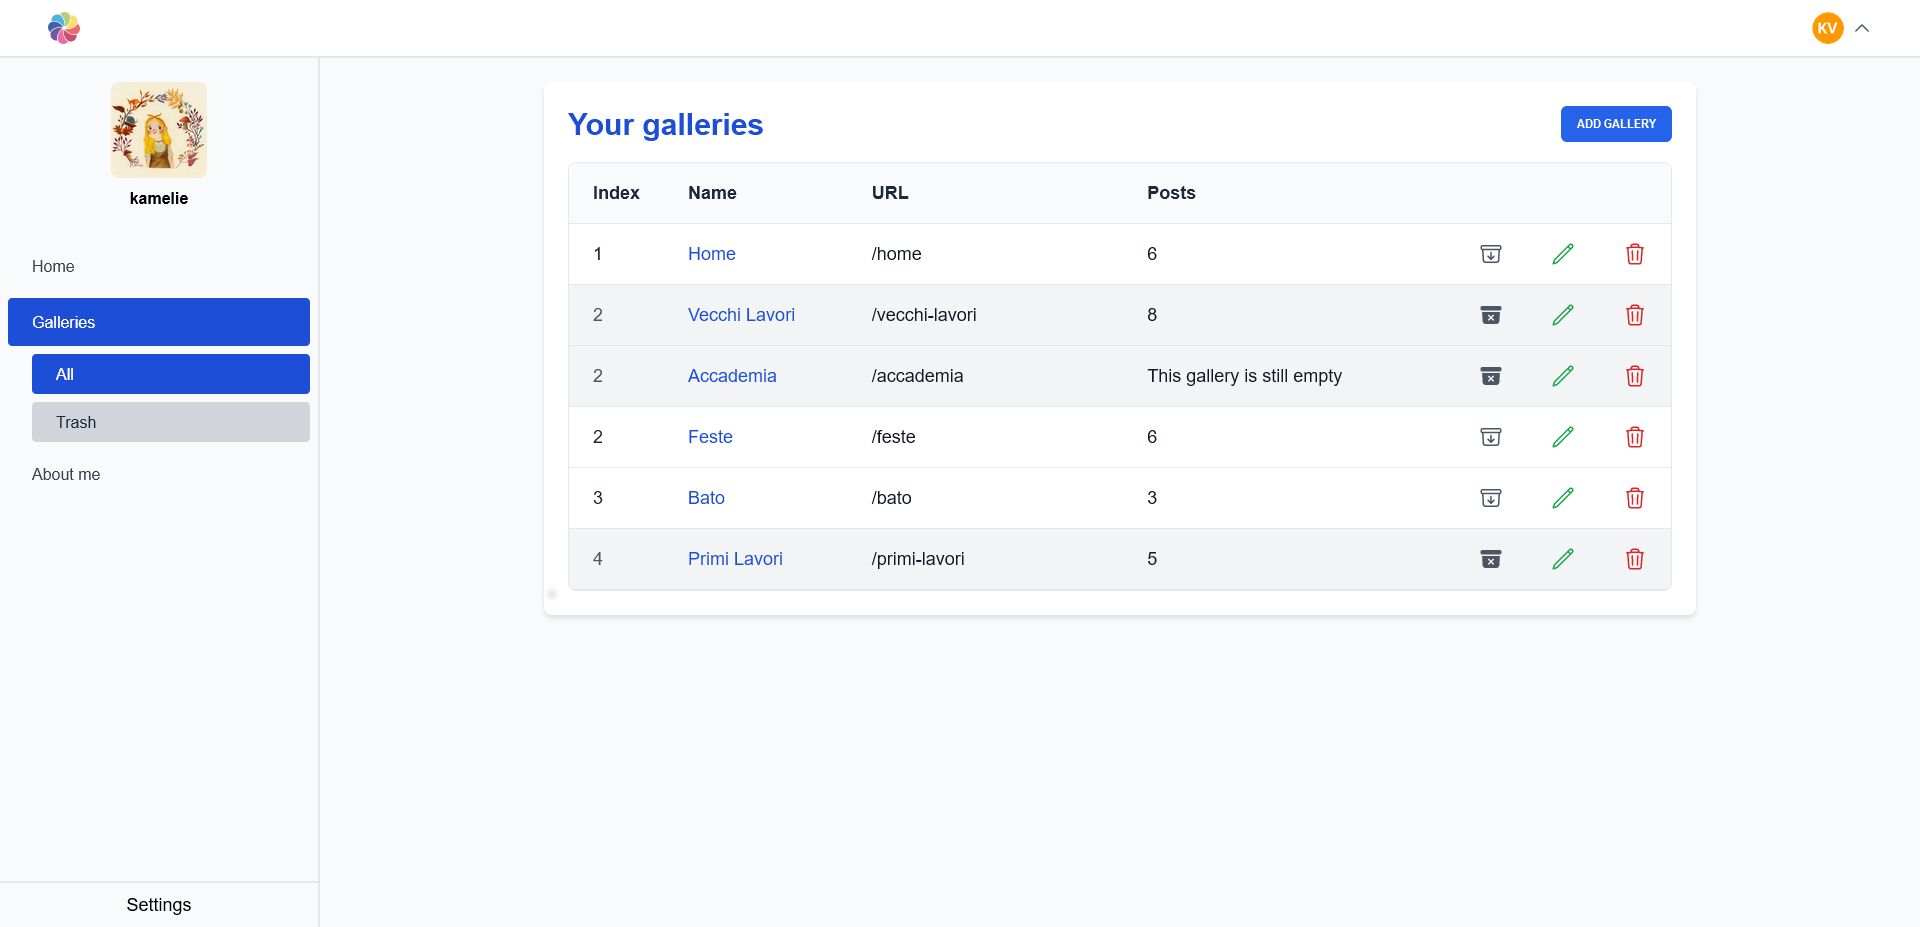
\includegraphics[width=1.0\linewidth]{figure/cms-g-all}}
	\caption{Pagina contenete la lista delle gallerie}
	\label{fig:cms-g-all}
\end{figure}

Durante il caricamento della pagina, viene eseguita l'azione \verb|getGalleries| dello store Pinia \verb|CMSStore|, la quale restituisce lo stato \verb|galleries|. Se lo stato non ha valori viene eseguita l'azione \verb|fetchGalleries| che effettua una richiesta GET all'URI dell'API \verb|v1/cms/portfolios/{portfolio}/galleries| per ottenere le gallerie del portfolio dell'utente e se essa ha successo verr\`a inizializzato lo stato \verb|galleries|. 

\subsubsection{Pagina di creazione di una galleria}
Attraverso il pulsante ``ADD GALLERY'' \`e possibile collegarsi alla pagina ``portfolio/new-gallery'' per compilare il modulo di creazione di una nuova galleria. Tale modulo \`e rappresentato dal componente Vue \verb|GalleryAdd.vue|:

\begin{figure}[htbp]
	\centering
	\fboxsep=0.5pt
	\fboxrule=0.5pt
	\fcolorbox{black}{black}{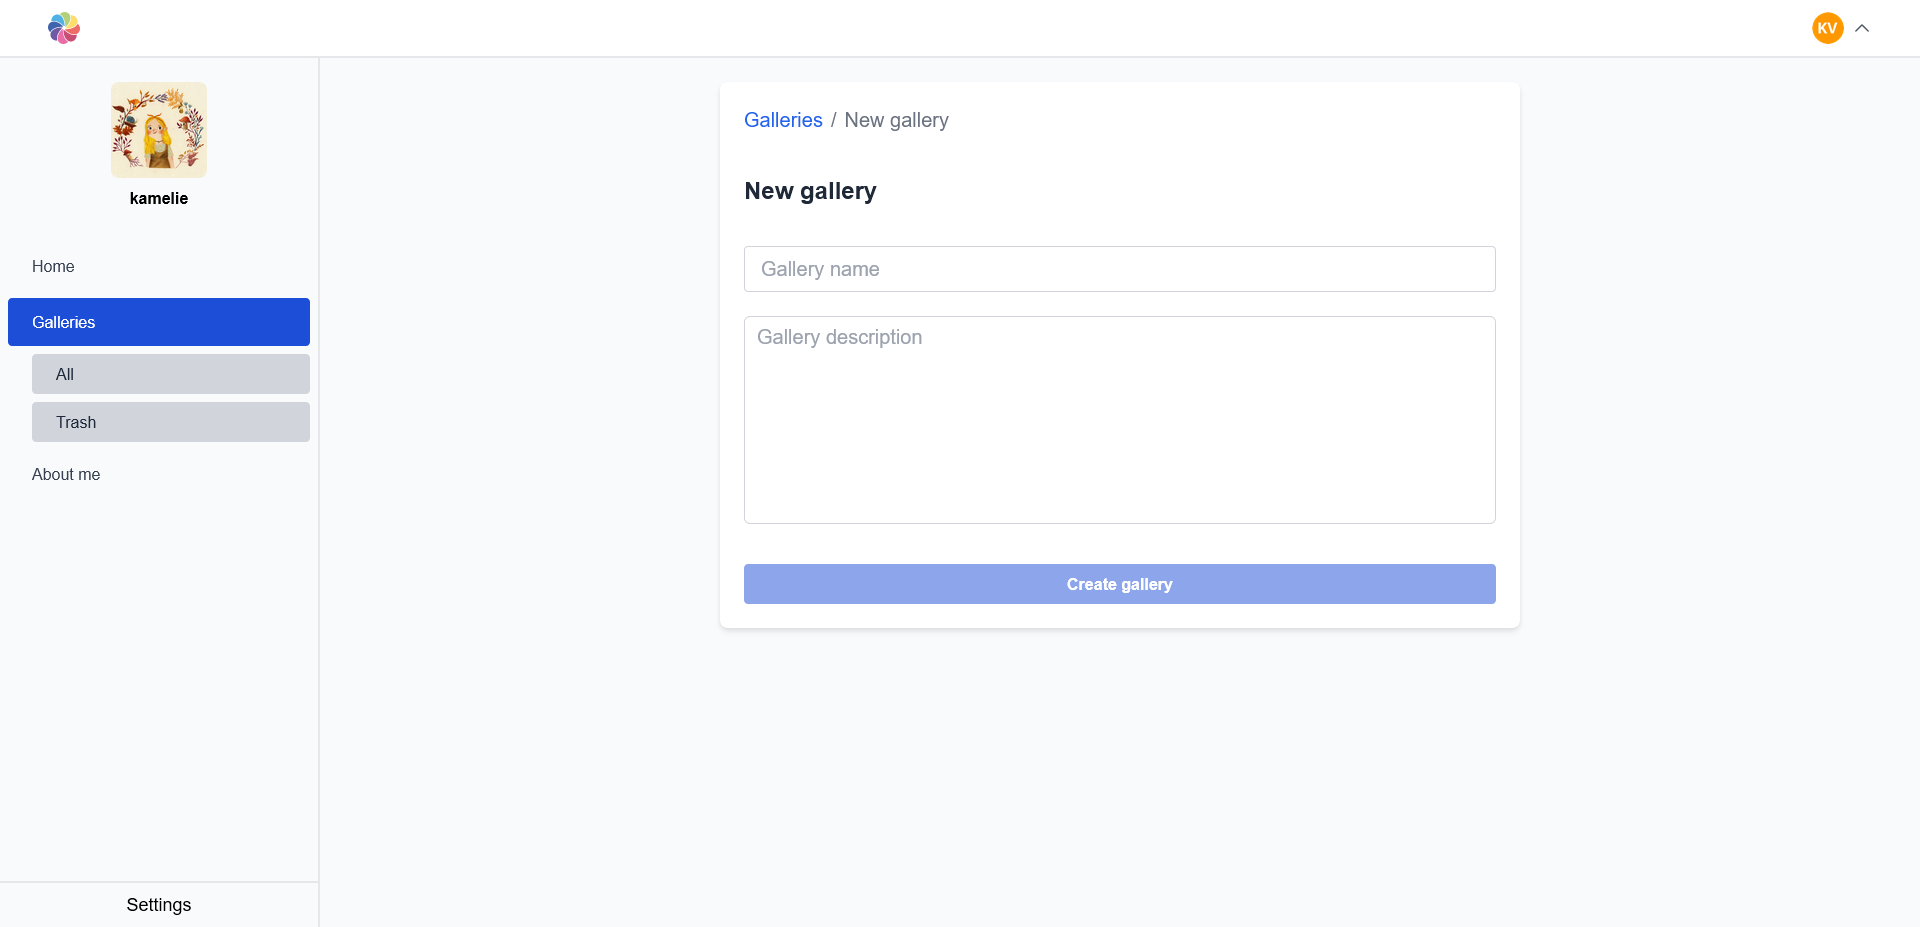
\includegraphics[width=1.0\linewidth]{figure/cms-g-new}}
	\caption{Pagina per l'aggiunta di una nuova galleria}
	\label{fig:cms-g-new}
\end{figure}

Una volta che l'utente avr\`a compilato ogni campo, il modulo potr\`a essere inviato. Sar\`a quindi possibile eseguire la funzione \verb|createGallery| la quale utilizza a sua volta l'azione \verb|createGallery| dello store Pinia \verb|CMSStore|. Tale azione invia i campi del modulo attraverso una richiesta POST all'URI dell'API \verb|v1/cms/portfolios/{portfolio}/galleries|.

Se la richiesta ha successo verr\`a aggiornato lo stato dell'applicazione, aggiungendo la nuova galleria alla lista, se inizializzata, delle gallerie e incrementando il numero di gallerie del portfolio.

Se la richiesta fallisce, vengono mostrati dei messaggi di errore al di sotto dei campi interessati in modo tale che l'utente possa correggerli.

Infine, una volta che il modulo \`e stato compilato ed elaborato correttamente, l'utente verr\`a reindirizzato alla pagina della galleria creata.

\subsubsection{Pagina per la visualizzazione di una galleria}
L'utente pu\`o collegarsi alla pagina ``portfolio/galleries/:slug'' cliccando il nome di una galleria in modo tale da visualizzarne il contenuto. Tale pagina \`e rappresentata dal componente Vue \verb|CMS\Gallery\GalleryView| (Figura~\ref{fig:cms-g-view}).

\begin{figure}[htbp]
	\centering
	\fboxsep=0.5pt
	\fboxrule=0.5pt
	\fcolorbox{black}{black}{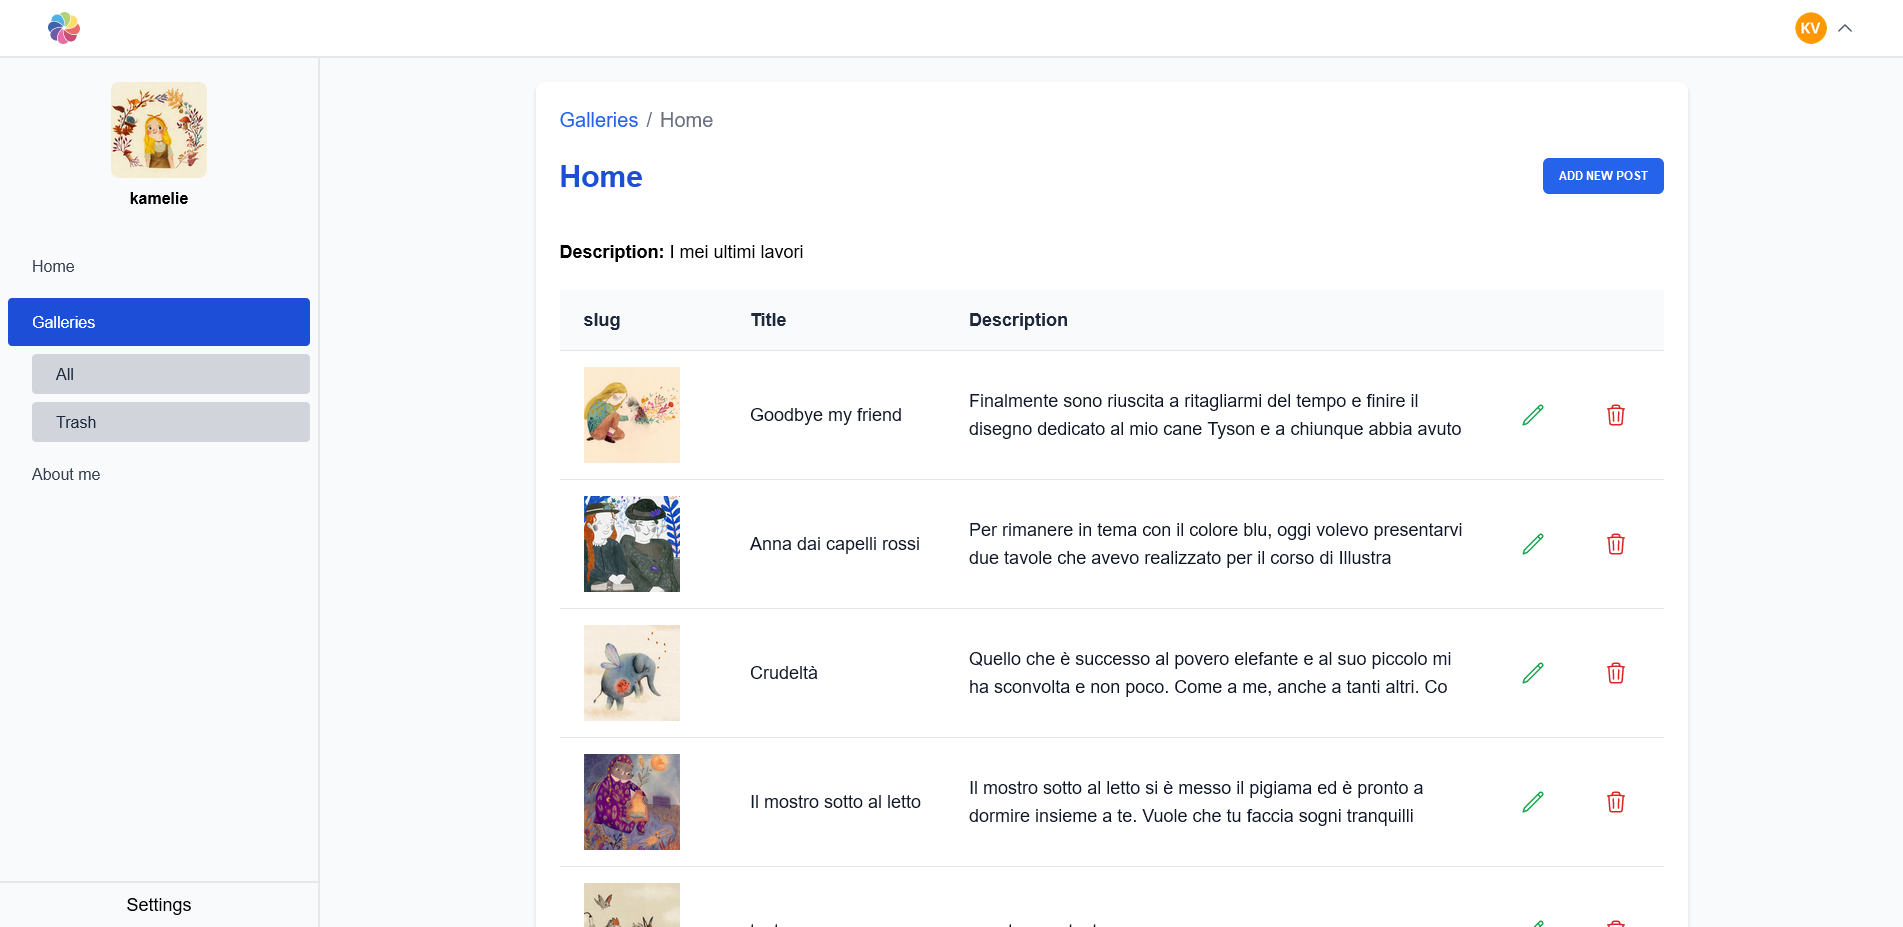
\includegraphics[width=1.0\linewidth]{figure/cms-g-view}}
	\caption{Pagina per la visualizzazione di una galleria}
	\label{fig:cms-g-view}
\end{figure}

Durante il caricamento della pagina, viene eseguita l'azione \verb|getGallery| dello store Pinia \verb|CMSStore|, la quale cerca nello stato \verb|galleries| la galleria con lo slug uguale a quello nel parametro dell'URL della pagina. Se lo stato non ha valori viene eseguita l'azione \verb|fetchGallery| che effettua una richiesta GET all'URI dell'API \verb|v1/cms/portfolios/{portfolio}/galleries/{gallery}| per ottenere la galleria.

Se lo slug non \`e valido, l'utente viene reindirizzato alla pagina ``not-found''.

\subsubsection{Pagina per l'aggiornamento di una galleria}
Tramite i pulsanti per la modifica di una galleria \`e possibile collegarsi alla pagina ``portfolio/galleries/:slug/edit'' per modificare il modulo di aggiornamento di una galleria. Tale modulo \`e rappresentato dal componente Vue \verb|GalleryEdit.vue|:

\begin{figure}[htbp]
	\centering
	\fboxsep=0.5pt
	\fboxrule=0.5pt
	\fcolorbox{black}{black}{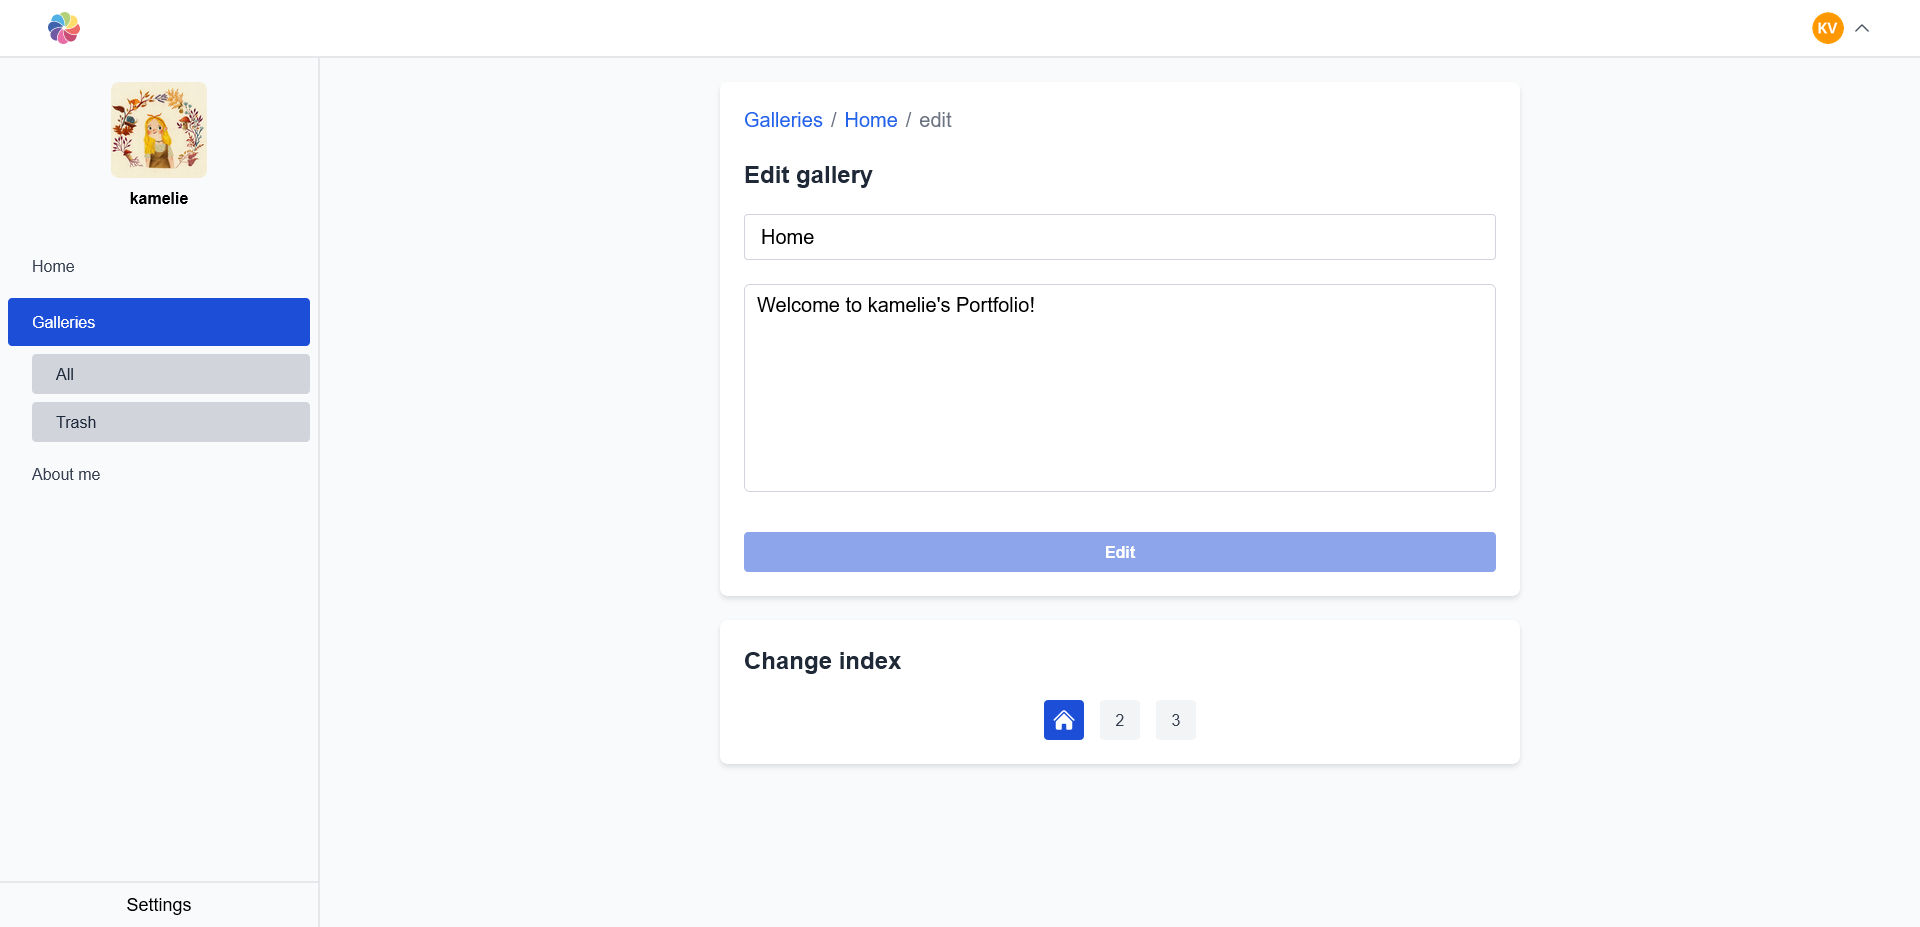
\includegraphics[width=1.0\linewidth]{figure/cms-g-update}}
	\caption{Pagina per la modifica di una galleria}
	\label{fig:cms-g-update}
\end{figure}

Durante il caricamento della pagina, viene eseguito il procedimento per ottenere la galleria corrente in modo tale da precompilare il modulo di modifica della galleria.

Una volta che l'utente avr\`a modificato almeno un campo, il modulo potr\`a essere inviato. Sar\`a quindi possibile eseguire la funzione \verb|editGallery| la quale utilizza a sua volta l'azione \verb|editGallery| dello store Pinia \verb|CMSStore|. Tale azione invia i campi del modulo attraverso una richiesta PATCH all'URI dell'API \verb|v1/cms/portfolios/{portfolio}/galleries/{gallery}|.

Se la richiesta ha successo, verr\`a aggiornato lo stato dell'applicazione, modificando la galleria nella lista, se inizializzata, delle gallerie.

Se la richiesta fallisce, vengono mostrati dei messaggi di errore al di sotto dei campi interessati in modo tale che l'utente possa correggerli.

Una volta che il modulo \`e stato compilato ed elaborato correttamente, verr\`a avvisato l'utente della corretta modifica tramite un messaggio di successo in cima al modulo  (Figura~\ref{fig:cms-g-update-success}).

Oltre alla modifica del nome e descrizione della galleria, se la galleria non \`e archiviata, l'utente pu\`o modificare l'indice della galleria attraverso una serie di pulsanti che utilizzando la funzione \verb|editGalleryIndex| la quale utilizza a sua volta l'azione \verb|editGalleryIndex| dello store Pinia \verb|CMSStore|.  Tale azione invia il nuovo indice attraverso una richiesta PATCH all'URI dell'API \verb|v1/cms/portfolios/{portfolio}/galleries/{gallery}/index|.

\begin{figure}[htbp]
	\centering
	\fboxsep=0.5pt
	\fboxrule=0.5pt
	\fcolorbox{black}{black}{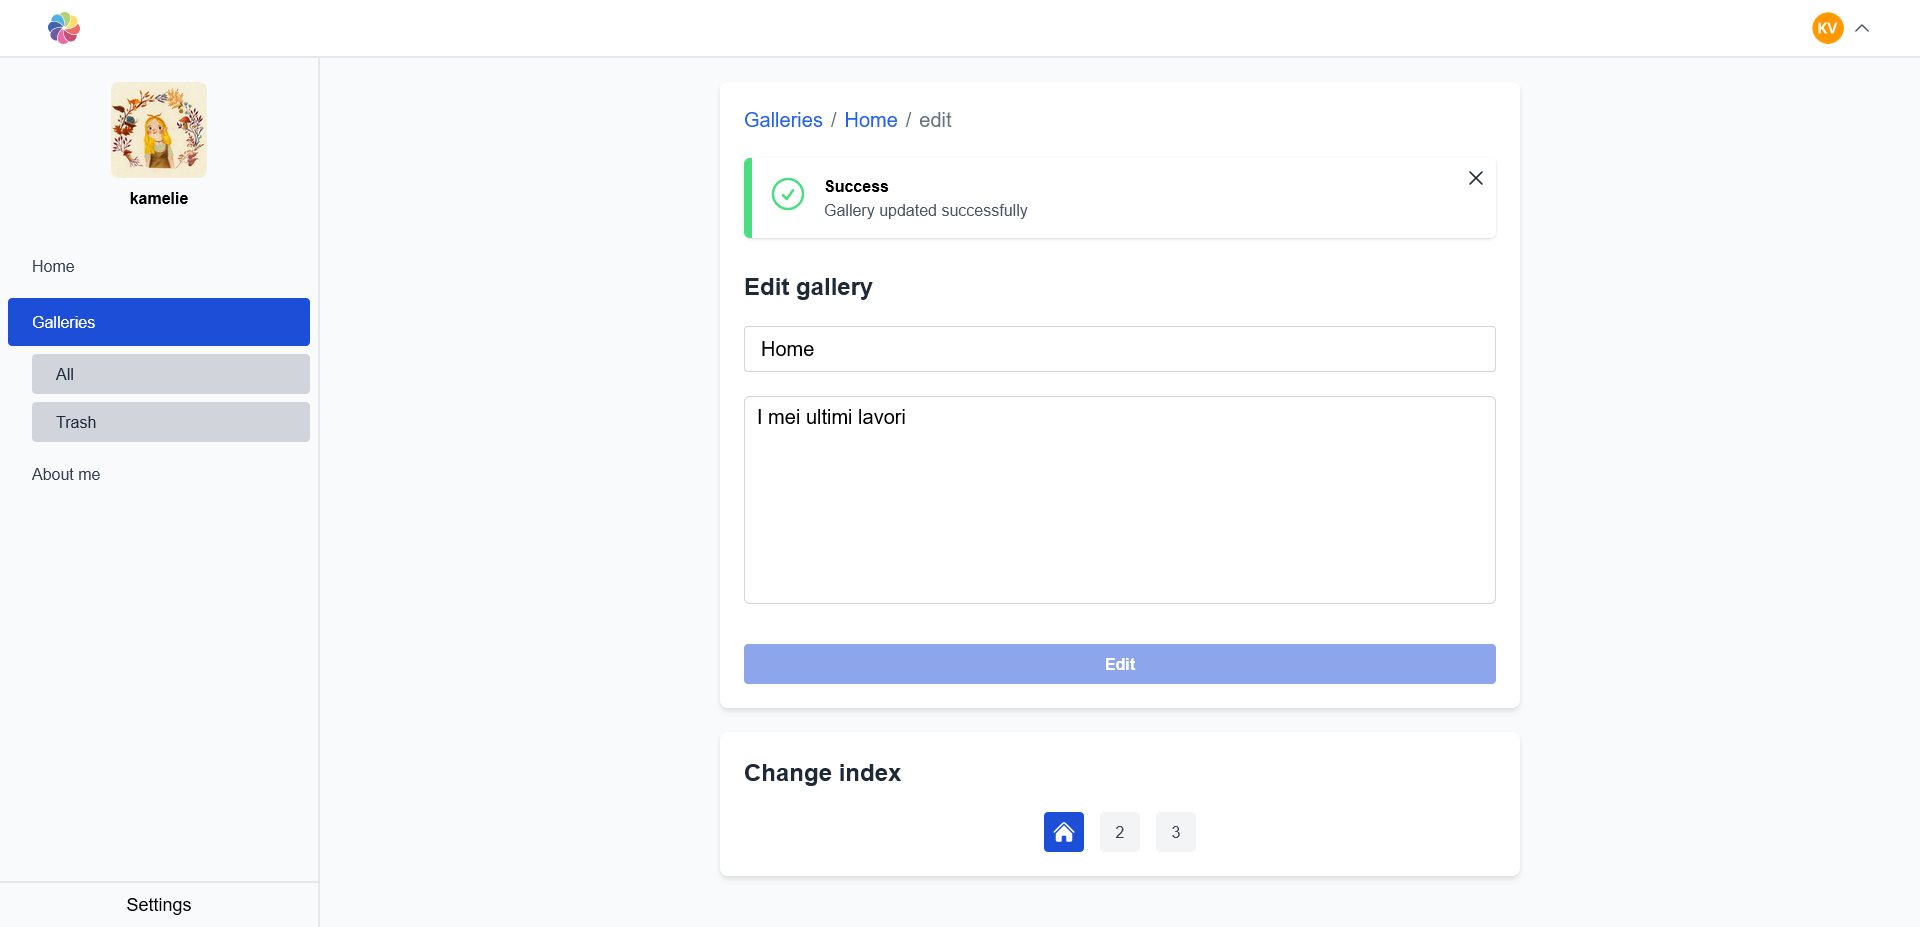
\includegraphics[width=1.0\linewidth]{figure/cms-g-update_success}}
	\caption{Pagina per la modifica di una galleria con un messaggio di successo}
	\label{fig:cms-g-update-success}
\end{figure}

\subsubsection{Pulsante per l'eliminazione di una galleria}
Tramite i pulsanti per l'eliminazione di una galleria \`e possibile utilizzare la funzione \verb|deleteGallery| per eliminare una galleria, la quale utilizza a sua volta l'azione \verb|deleteGallery| dello store Pinia \verb|CMSStore|. Tale azione effettua una richiesta DELETE all'URI dell'API \verb|v1/cms/portfolios/{portfolio}/galleries/{gallery}| e se essa ha successo verr\`a aggiornato lo stato dell'applicazione, rimuovendo la galleria dalla lista, se inizializzata, delle gallerie, inserendola nella lista, se inizializzata, delle gallerie eliminate e decrementando il numero di gallerie del portfolio. 


\subsection{Archiviazione gallerie}
\subsubsection{Laravel Route}
Per implementare l'archiviazione di una galleria \`e stata definita una route nel file \verb|routes\api\v1\cms.php|:
\begin{lstlisting}[caption={Route per l'archiviazione di una galleria}, label={lst:route_g_arch}]
Route::prefix('portfolios/{portfolio}/galleries/{gallery}')
	->group(function () {
		Route::patch(
			'archive', [GalleryArchiveController::class, 'update']
		);
		...
	});
\end{lstlisting}

\subsubsection{GalleryArchiveController@update}
Il metodo \verb|update| della classe \verb|GalleryArchiveController| ha come parametri il portfolio e la galleria.

Se la galleria \`e pubblica vengono decrementati gli indici delle gallerie pubbliche che hanno un indice maggiore della galleria da archiviare mentre il suo l'indice rimane invariato in modo tale da poterne ripristinare la posizione una volta disarchiviata.

Se la galleria \`e archiviata vengono incrementati gli indici delle gallerie pubbliche che hanno un indice maggiore della galleria da disarchiviare. Nel caso in cui l'indice della galleria fosse maggiore del numero di gallerie pubbliche, viene assegnato come indice della galleria il numero di gallerie pubbliche incrementato di uno.

Il metodo restituisce come risposta le informazioni di tutte gallerie e il messaggio ``Gallery archived successfully'', se \`e stata archiviata, o ``Gallery unarchived successfully'', se \`e stata disarchiviata.

\subsection{Ripristino ed eliminazione definitiva}
Per implementare l'eliminazione e ripristino di una galleria sono state definite tre route nel file \verb|routes\api\v1\cms.php|. (Codice~\ref{lst:route_g_del})

\begin{lstlisting}[caption={Route per la gestione delle gallerie eliminate}, label={lst:route_g_del}]
Route::get(
	'portfolios/{portfolio}/galleries/deleted',
	[GalleryDeleteController::class, 'index']
);

Route::prefix('portfolios/{portfolio}/galleries/{gallery}')
	->group(function () {
		...
		Route::patch(
			'delete',
			[GalleryDeleteController::class, 'update']
		);
		Route::delete(
			'delete',
			[GalleryDeleteController::class, 'destroy']
		);
	});
\end{lstlisting}


La prima permette di ottenere la lista di gallerie eliminate nel portfolio, mentre le altre due gestiscono il ripristino e l'eliminazione definitiva, rispettivamente.
\subsubsection{Pagina delle gallerie eliminate}
Per visualizzare e gestire le gallerie eliminate, l'utente si collega alla pagina ``portfolio/deleted-galleries''. Tale pagina \`e rappresentata dal componente Vue \verb|GalleriesDeletedView.vue| (Figura~\ref{fig:cms-g-del}).

\begin{figure}[htbp]
	\centering
	\fboxsep=0.5pt
	\fboxrule=0.5pt
	\fcolorbox{black}{black}{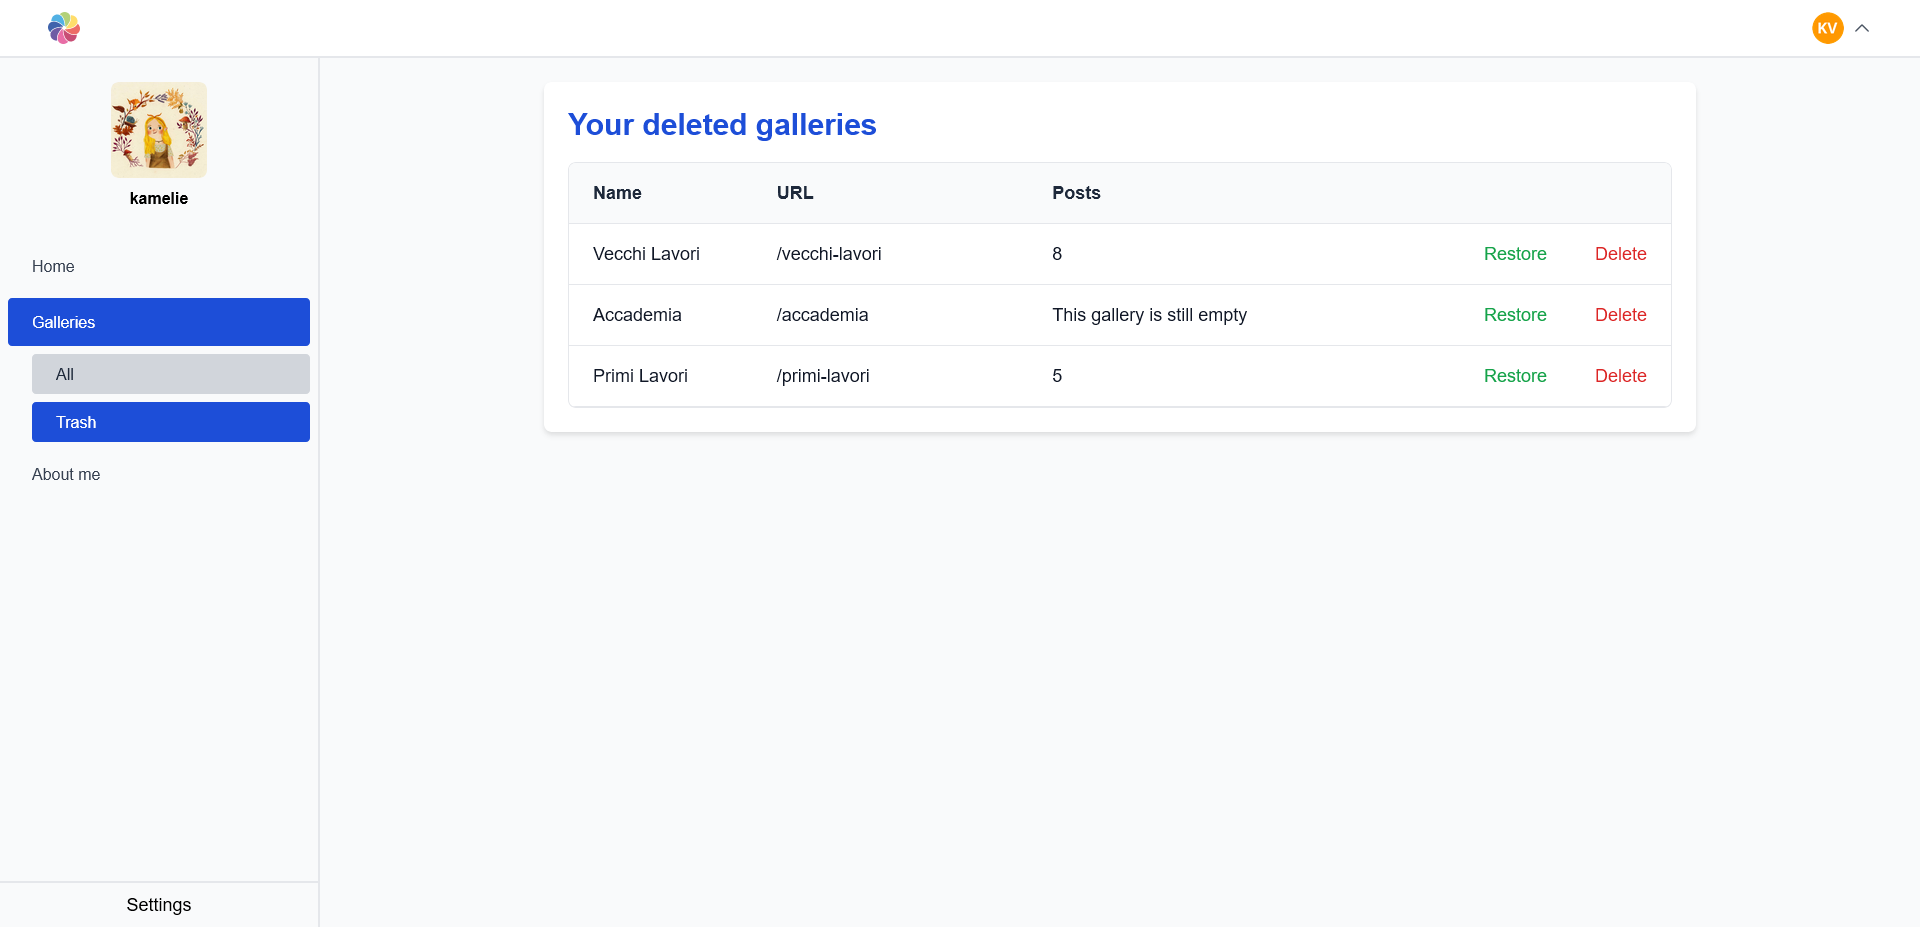
\includegraphics[width=1.0\linewidth]{figure/cms-g-del}}
	\caption{Pagina contenete la lista delle gallerie eliminate}
	\label{fig:cms-g-del}
\end{figure}



Durante il caricamento della pagina, viene eseguita l'azione \verb|getDeletedGalleries| dello store Pinia \verb|CMSStore|, la quale restituisce lo stato \verb|deletedGalleries|. Se lo stato non ha attributi viene eseguita l'azione \verb|fetchDeletedGalleries| che effettua una richiesta GET all'URI dell'API \verb|v1/cms/portfolios/{portfolio}/galleries/deleted| per ottenere le gallerie eliminate del portfolio utente e se essa ha successo verr\`a inizializzato lo stato \verb|deletedGalleries|. 

\subsection{Gestione post}
\subsubsection{Laravel Route}
Per implementare le operazioni principali per la gestione dei post sono state definite, attraverso il metodo \verb|apiResource| della classe \verb|Route|, le route per l'utilizzo dei metodi \verb|index|, \verb|store|, \verb|show|, e \verb|destroy| della classe \verb|PostController| e, attraverso il metodo \verb|post|, la route per l'utilizzo del metodo \verb|update| con il metodo HTTP POST nel file \verb|routes\api\v1\cms.php|:
\begin{lstlisting}[caption={Route operazioni principali per la gestione dei post}, label={lst:route-cms-p}]
Route::apiResource(
	'portfolios.galleries.posts',
	PostController::class
)->except(['update']);

Route::post(
	'portfolios/{portfolio}/galleries/{gallery}/posts/{post}',
	[PostController::class, 'update']
);
\end{lstlisting}

\subsubsection{PostController@store}
Il metodo \verb|store| della classe \verb|PostController| ha come parametri una richiesta di tipo \verb|CreatePostRequest|, il portfolio e la gallery. La classe \verb|CreatePostRequest| si occupa di convalidare ogni richiesta, verificando che siano presenti i campi ``title'', ``description'' e ``media'', necessari per effettuare la creazione del post e che rispettino le regole definite nella classe \verb|PostRules|. 

Se la richiesta \`e valida viene eseguito il metodo, il quale:
\begin{itemize}
	\item Crea uno slug unico per il post utilizzando il trait \verb|generateUniqueSlug| della classe \verb|GenerateSlug|.
	\item Crea un nuovo post nella base di dati.
	\item Salva il media della richiesta nella cartella \verb|'posts/' . $portfolio->id| utilizzando come nome del file lo slug generato.
	\item Crea una versione 1200x1200 del media e lo salva nella cartella \verb|'posts/' . $portfolio->id . '/thumbnail'|
\end{itemize} 
Il metodo restituisce come risposta le informazioni sul post creato, secondo quanto specificato nella classe \verb|PostResource|:
\begin{lstlisting}[caption={Risposta di successo creazione post}, label={lst:response_success_registration}]
{
	"status": "success",
	"data": {
		"message": "Post created successfully",
		"post": {
			"title": "...",
			"description": "...",
			"slug": "aqSuhkwkOzSL",
			"thumbnail": "media/posts/1/thumbnail/aqSuhkwkOzSL.png",
			"media": "media/posts/1/aqSuhkwkOzSL.png"
		}
	}
}
\end{lstlisting}

\subsubsection{PostController@destroy}
Il metodo \verb|destroy| della classe \verb|PostController| ha come parametri il portfolio, la gallery e il post. Tale metodo si occupa di eliminare i media del post dal filesystem e di eliminare definitivamente il post.

Il metodo restituisce come risposta il messaggio \textit{``Post deleted successfully''}.


\subsubsection{PostController@update}
Il metodo \verb|update| della classe \verb|PostController| ha come parametri  una richiesta di tipo \verb|UpdatePostRequest|, il portfolio, la gallery e il post. Tale metodo si occupa di eliminare i media del post dal filesystem e di eliminare definitivamente il post. La classe \verb|UpdatePostRequest| si occupa di convalidare ogni richiesta, verificando che siano presenti i campi ``title'', ``description'', necessari per effettuare l'aggiornamento del post, che rispettino le regole definite nella classe \verb|PostRules| e che il campo ``media'', se presente, sia un immagine.

Se la richiesta \`e valida viene eseguito il metodo, il quale modifica il titolo e la descrizione del post. Se \`e presente il media nella richiesta, elimina i media del post dal filesystem sostituendoli con quelli del nuovo media.

Il metodo restituisce come risposta le informazioni sul post modificato e il messaggio \textit{``Post updated successfully''}.

\subsubsection{Pagina di creazione di un post}
Attraverso il pulsante ``ADD NEW POST'' \`e possibile collegarsi alla pagina ``portfolio/galleries/:slug/new-post'' per compilare il modulo di creazione di un nuovo post. Tale modulo \`e rappresentato dal componente Vue \verb|PostAdd.vue|:

\begin{figure}[htbp]
	\centering
	\fboxsep=0.5pt
	\fboxrule=0.5pt
	\fcolorbox{black}{black}{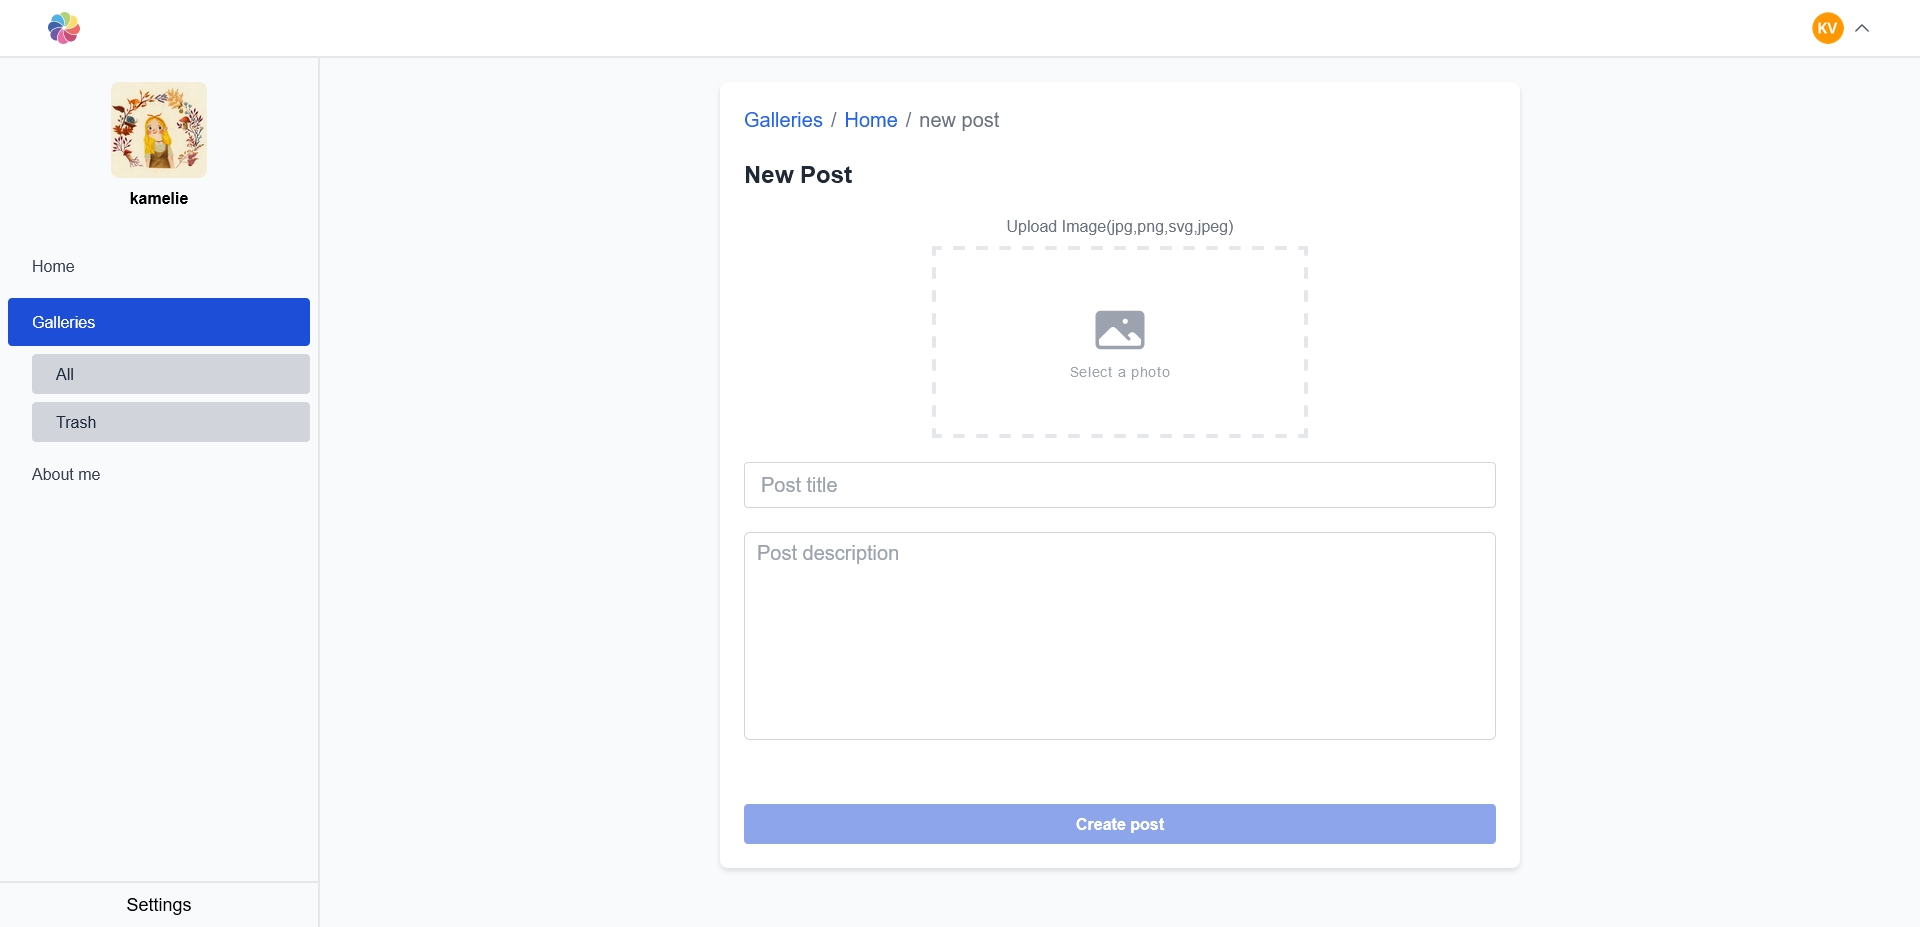
\includegraphics[width=1.0\linewidth]{figure/cms-p-new}}
	\caption{Pagina per l'aggiunta di un nuovo post}
	\label{fig:fig:cms-p-new}
\end{figure}

Una volta che l'utente avr\`a compilato ogni campo (Figura~\ref{fig:cms-p-new1}), il modulo potr\`a essere inviato. Sar\`a quindi possibile eseguire la funzione \verb|createPost| la quale utilizza a sua volta l'azione \verb|createPost| dello store Pinia \verb|CMSStore|. Tale azione invia i campi del modulo attraverso una richiesta POST all'URI dell'API \verb|v1/cms/portfolios/{portfolio}/galleries/{gallery}/posts| e se essa ha successo verr\`a aggiornato lo stato dell'applicazione, aggiungendo il post creato alla lista, se inizializzata, dei post della rispettiva galleria.

Infine, una volta che il modulo \`e stato compilato ed elaborato correttamente, l'utente verr\`a reindirizzato alla pagina della galleria nella quale \`e presente il post creato.


\begin{figure}[htbp]
	\centering
	\fboxsep=0.5pt
	\fboxrule=0.5pt
	\fcolorbox{black}{black}{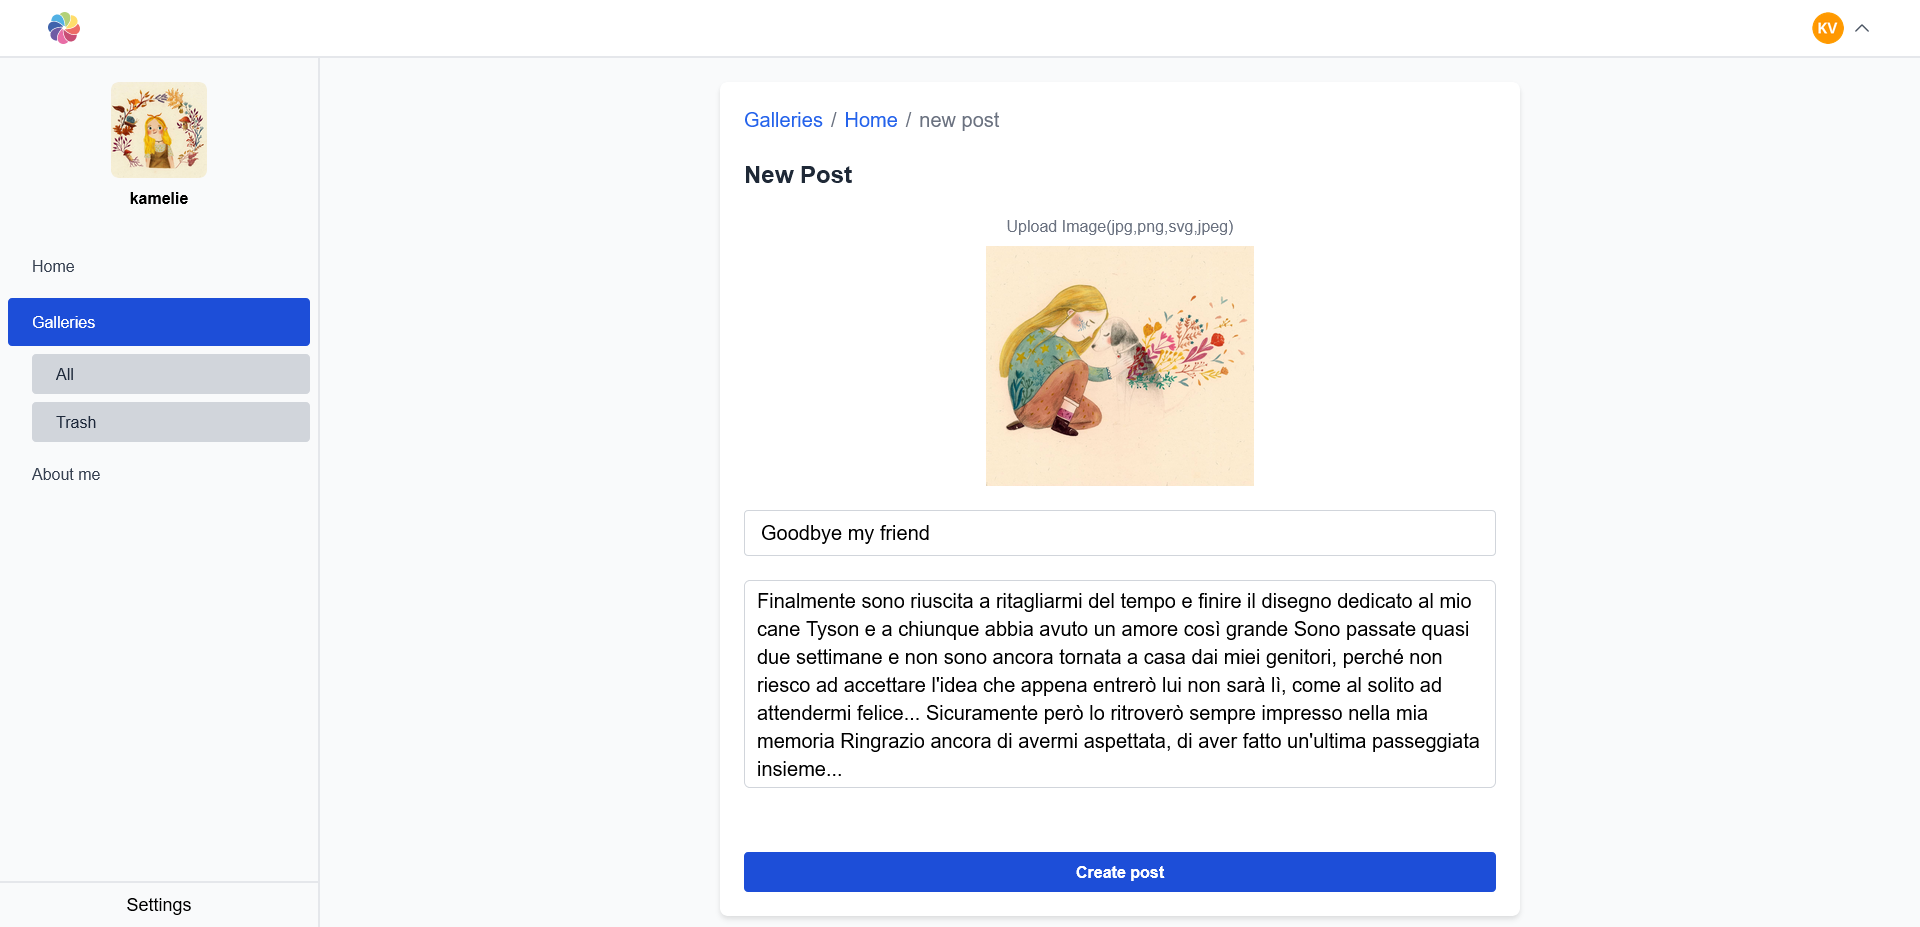
\includegraphics[width=1.0\linewidth]{figure/cms-p-new2}}
	\caption{Pagina per l'aggiunta di un nuovo post con il modulo compilato}
	\label{fig:cms-p-new1}
\end{figure}
%%

\section{Visualizzazione portfolio}
L'implementazione della visualizzazione di un portfolio consiste nella realizzazione di tutte le componenti necessarie per la navigazione tra le sezioni di un portfolio pubblico, ossia n\'e archiviato n\'e eliminato.
\subsection{Portfolio pubblico}
\subsubsection{Laravel Route}
Per ottenere le informazioni su un portfolio portfolio pubblico \`e stata definita una route nel file \verb|routes\api\v1\api.php|:
\begin{lstlisting}[caption={Route per ottenere un portfolio pubblico}, label={lst:route_public_portfolio}]
Route::get(
	'portfolios/{portfolio}', 
	[PortfolioController::class, 'show']
);
\end{lstlisting}

\subsubsection{PortfolioController@show}
Il metodo \verb|show| della classe \verb|Public\PortfolioController| ha come parametri una richiesta di tipo \verb|ShowPublicPortfolioRequest| e un portfolio. La classe \verb|ShowPublicPortfolioRequest| si occupa di convalidare ogni richiesta, verificando il portfolio che si vuole visualizzare non \`e archiviato e che abbia almeno una galleria.

Se la richiesta \`e valida, il metodo restituisce come risultato le informazioni del portfolio, secondo quanto specificato nella classe \verb|PortfolioPublicResource|:
\begin{lstlisting}[caption={Risposta di successo portfolio pubblico}, label={lst:response_success_public_pf}]
{
	"status": "success",
	"data": {
		"portfolio": {
			"name": "kamelie",
			"icon": "media/portfolio/icon/icon-1.png",
			"home": "home",
			"sections": [
				{
					"category": "gallery",
					"slug": "home",
					"name": "Home"
				},
				...
				{
					"category": "about-me",
					"slug": "about-me",
					"name": "About me"
				}
			]
		}
	}
}
\end{lstlisting}

\subsubsection{Layout portfolio}
Il layout per le sezioni del portfolio pubblico \`e rappresentato dal componente Vue \verb|PublicPortfolioLayout.vue| ed \`e composto da un pannello, nel quale vengono mostrate l'icona, il nome e la barra di navigazione del portfolio, e da una \verb|RouterView| nella quale verr\`a montato il contenuto della sezione del portfolio.
\subsection{Sezione principale}
\subsubsection{Laravel Route}
Per ottenere le informazioni sulla sezione principale di un portfolio pubblico \`e stata definita una route nel file \verb|routes\api\v1\api.php|:
\begin{lstlisting}[caption={Route ottenere la sezione principale di un portfolio pubblico}, label={lst:route_public_portfolio_home}]
Route::get(
	'portfolios/{portfolio}/home',
	[PortfolioHomeController::class, 'show']
);
\end{lstlisting}

\subsubsection{PortfolioHomeController@show}
Il metodo \verb|show| della classe \verb|PortfolioHomeController| ha come parametri una richiesta di tipo \verb|ShowPublicPortfolioRequest| e un portfolio.

Se la richiesta \`e valida, il metodo restituisce come risultato la galleria con indice uguale ad uno, e i suoi relativi post, secondo quanto specificato nella classe \verb|PublicGalleryResource|:
\begin{lstlisting}[caption={Risposta di successo sezione principale di un portfolio pubblico}, label={lst:response_success_registration}]
{
	"status": "success",
	"data": {
		"section": {
			"category": "gallery",
			"slug": "home",
			"name": "Home",
			"description": "I mei ultimi lavori",
			"posts": [
				{
					"title": "..",
					"description": "...",
					"slug": "0KiZfYDgaItf",
					"thumbnail": "...",
					"media": "..."
				},
				...
			]
		}
	}
}
\end{lstlisting}

\subsubsection{Pagina principale del portfolio}
Per la visualizzazione di un portfolio pubblico, un utente si collega alla pagina ``:name'' della piattaforma. Tale pagina \`e rappresentata dal componente Vue \verb|PublicPortfolioSection.vue|:
\begin{figure}[htbp]
	\centering
	\fboxsep=0.5pt
	\fboxrule=0.5pt
	\fcolorbox{black}{black}{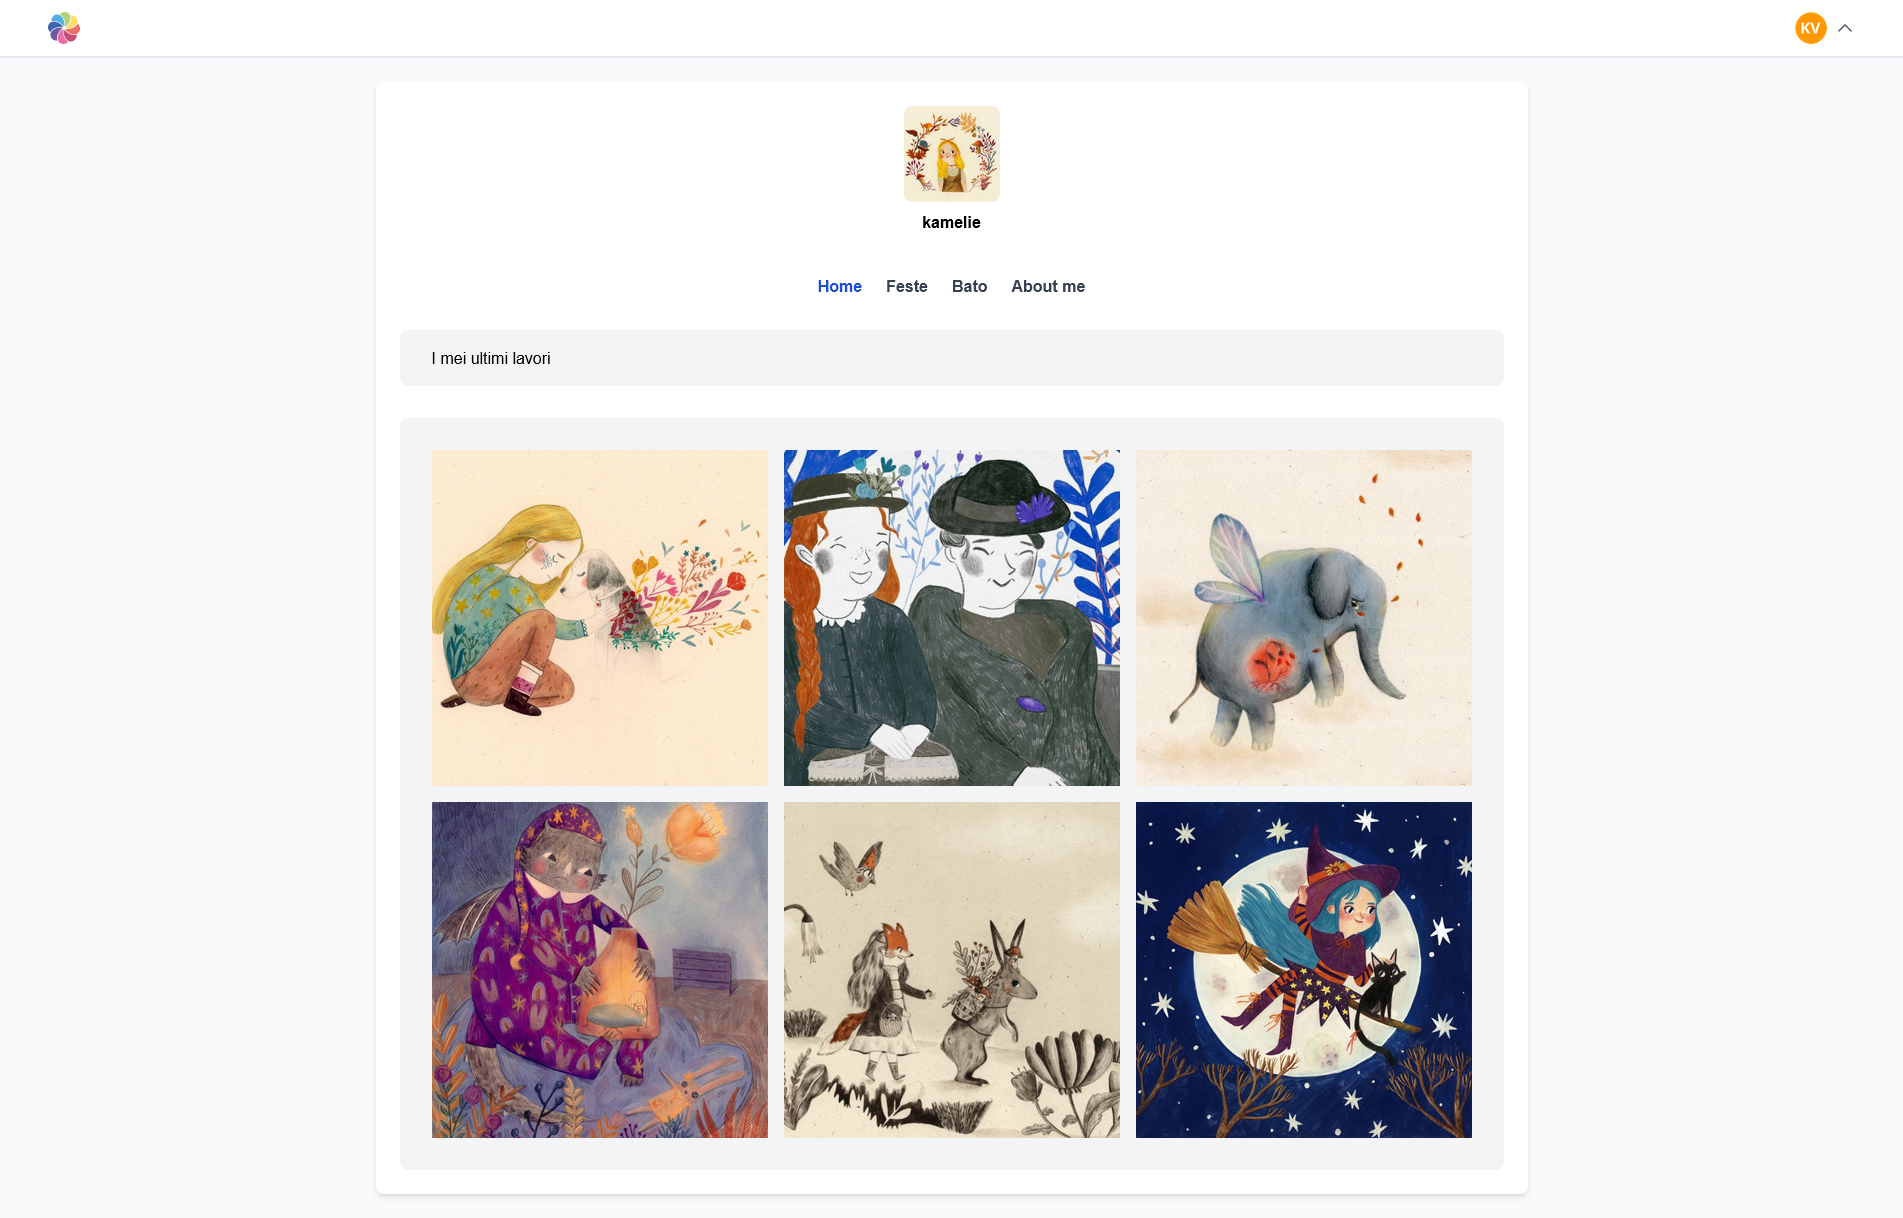
\includegraphics[width=1.0\linewidth]{figure/p-h-view}}
	\caption{Pagina principale portfolio}
	\label{fig:p-h-view}
\end{figure}


Durante il caricamento della pagina, viene eseguita la funzione \verb|setup()|, la quale verifica se nell'URL \`e presente il parametro ``slug'' di sezione. Se l'utente si trova nella sezione principale della piattaforma, tale parametro sar\`a assente. La funzione controlla, quindi, se nello stato \verb|portfolio|, dello store Pinia \verb|PortfolioStore|, sono presenti i post della prima sezione, la quale rappresenta la homepage del portfolio. Se tali post non sono presenti, viene eseguita l'azione \verb|fetchHome| che effettua una richiesta GET all'URI dell'API \verb|v1/portfolios/{portfolio}/home| per ottenere la
galleria del homepage del portfolio e se essa ha successo verr\`a aggiunta la galleria nella lista \verb|sections| dello stato \verb|portfolio|.

Una volta caricato il contenuto della galleria, per vedere il contenuto di un post, l'utente potr\`a cliccarci sopra, in modo tale da espandere il post e mostrare anche il suo titolo e descrizione (Figura~\ref{fig:p-h-view-p}).

\begin{figure}[htbp]
	\centering
	\fboxsep=0.5pt
	\fboxrule=0.5pt
	\fcolorbox{black}{black}{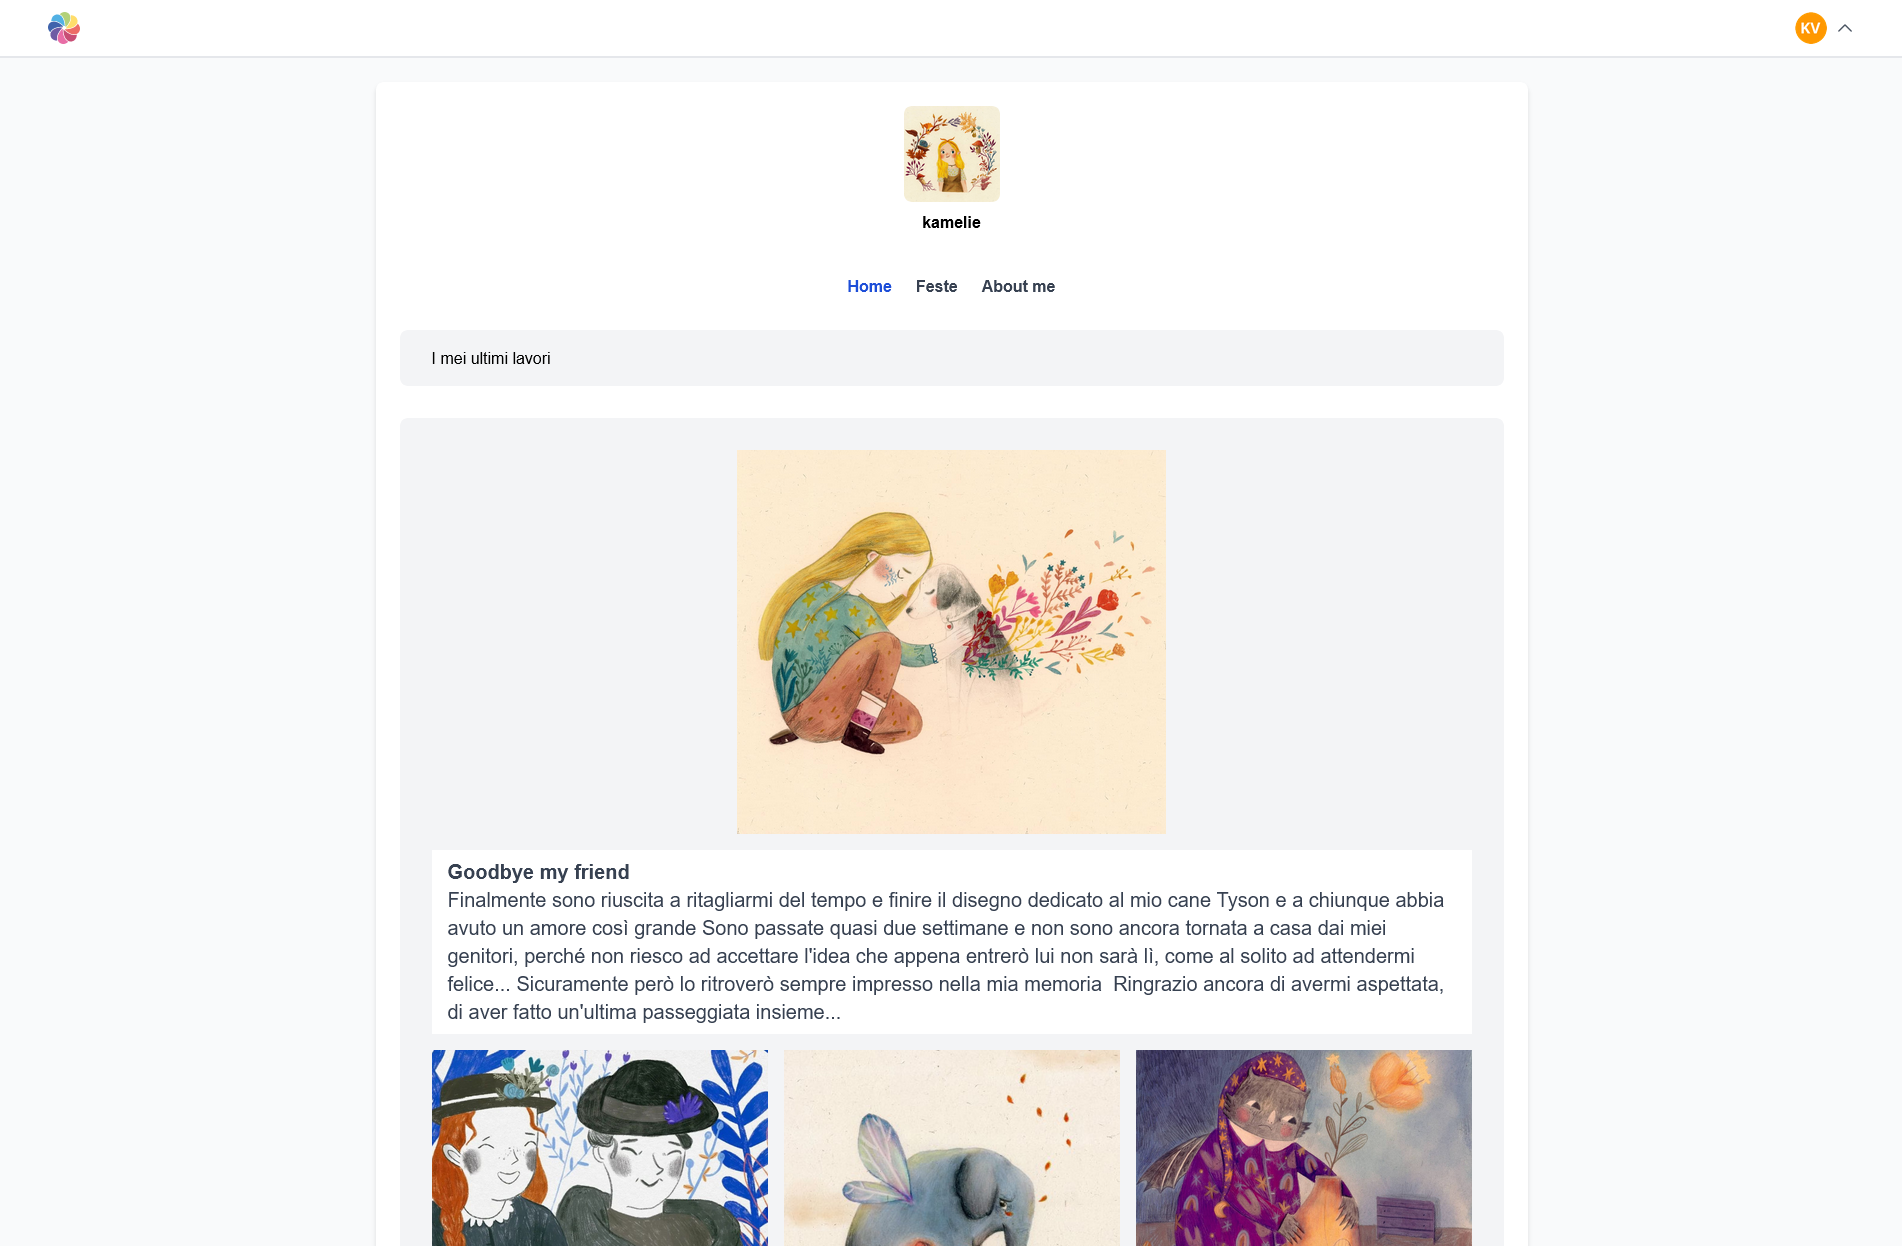
\includegraphics[width=1.0\linewidth]{figure/p-h-view-p}}
	\caption{Visualizzazione post}
	\label{fig:p-h-view-p}
\end{figure}

\subsection{Visualizzazione gallerie}
\subsubsection{Laravel Route}
Per ottenere le informazioni su una galleria di un portfolio pubblico \`e stata definita una route nel file \verb|routes\api\v1\api.php| (Codice~\ref{lst:route_public_portfolio_gallery}).

\begin{lstlisting}[caption={Route ottenere la una galleria di un portfolio pubblico}, label={lst:route_public_portfolio_gallery}]
Route::get(
	'portfolios/{portfolio}/galleries/{gallery}',
	[GalleryController::class, 'show']
);
\end{lstlisting}

\subsubsection{GalleryController@show}
Il metodo \verb|show| della classe \verb|Public\GalleryController| ha come parametri una richiesta di tipo \verb|ShowPublicPortfolioRequest| e un portfolio.

Se la richiesta \`e valida, il metodo restituisce come risultato la galleria e i suoi relativi post. 

\subsubsection{Pagina contenete una galleria}
Per la visualizzazione di una sezione del portfolio pubblico, un utente si collega alla pagina ``:name/:slug'' della piattaforma. Tale pagina \`e rappresentata dal componente Vue \verb|Portfolio\GalleryView.vue|:
\begin{figure}[htbp]
	\centering
	\fboxsep=0.5pt
	\fboxrule=0.5pt
	\fcolorbox{black}{black}{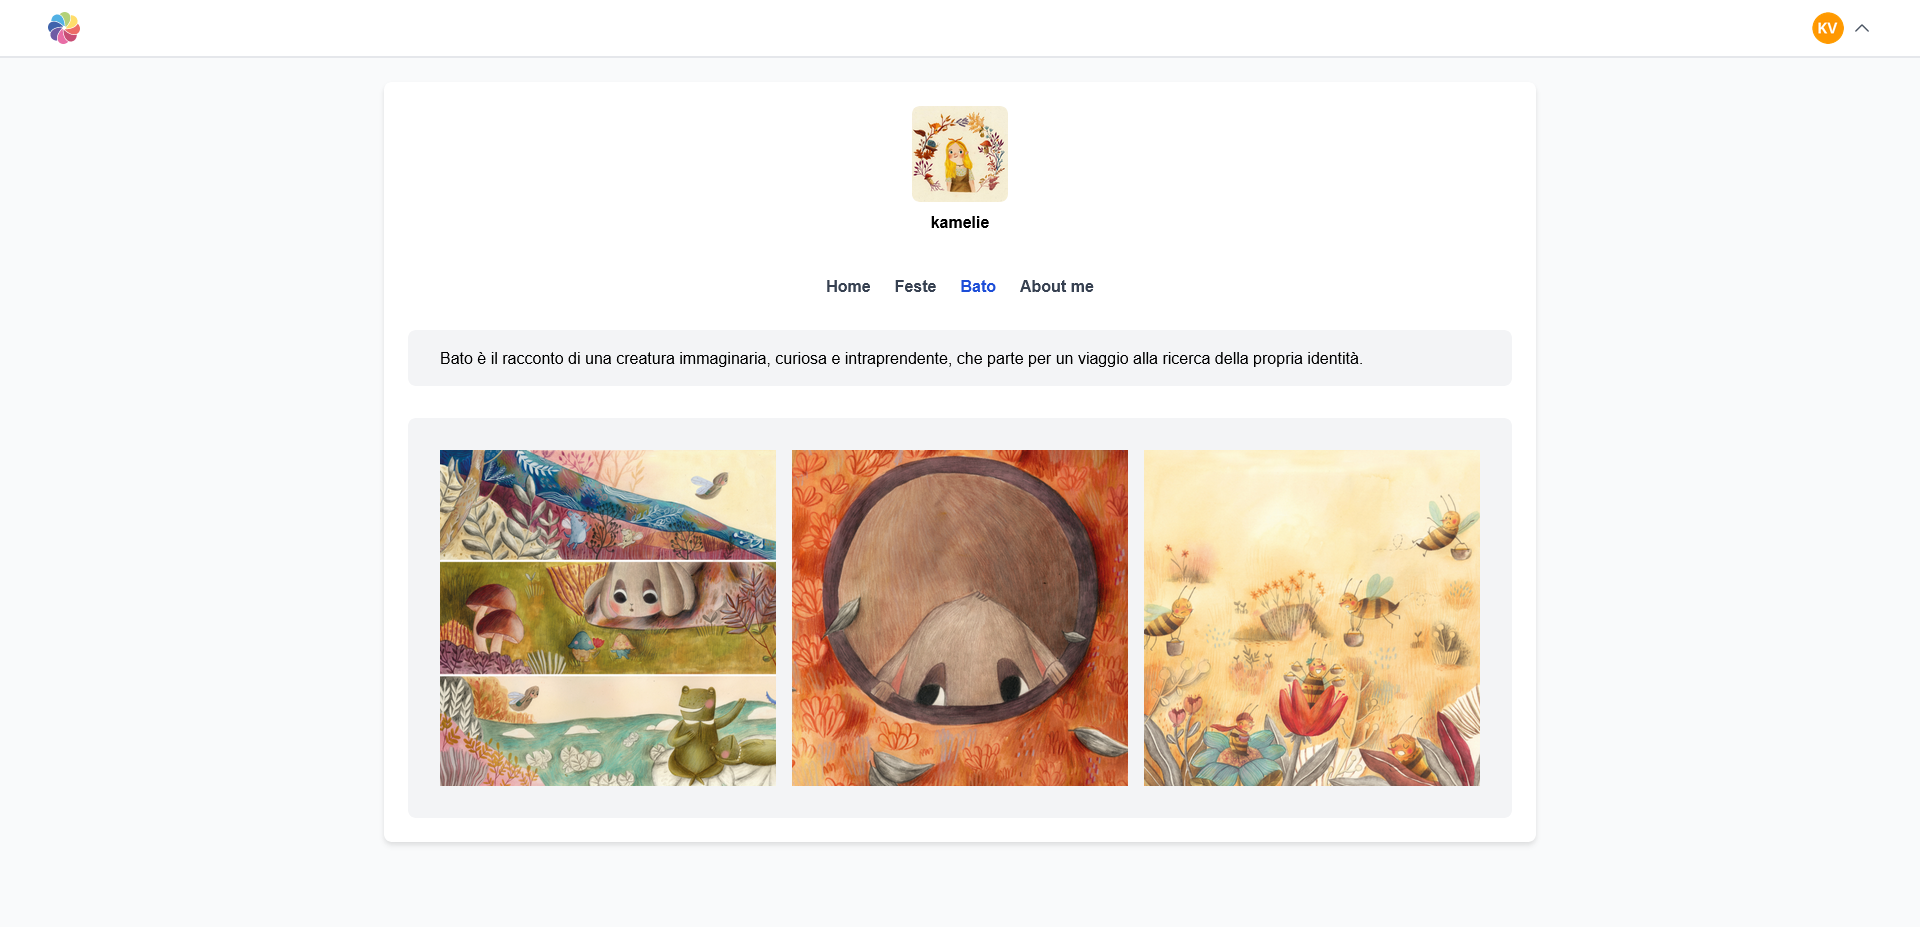
\includegraphics[width=1.0\linewidth]{figure/p-g-view}}
	\caption{Pagina del portfolio pubblico contenete una galleria}
	\label{fig:p-g-view}
\end{figure}


Durante il caricamento della pagina, viene eseguita la funzione \verb|setup()|, la quale verifica se nell'URL \`e presente il parametro ``slug'' di sezione. In tal caso, verifica la tipologia di sezione e se corrisponde a ``gallery'', viene eseguito la funzione \verb|getGallery|. Tale funzione controlla se nello stato \verb|portfolio|, dello store Pinia \verb|PortfolioStore|, sono presenti i post della sezione corrente. Se tali post non sono presenti, viene eseguita l'azione \verb|fetchGallery| che effettua una richiesta GET all'URI dell'API \verb|v1/portfolios/{portfolio}/galleries/{gallery}| per ottenere la galleria della sezione corrente.

Se la richiesta ha successo verr\`a aggiunta la galleria nella lista \verb|sections| dello stato \verb|portfolio|.

Se la richiesta fallisce, in quanto la sezione, relativa allo slug presente nel parametro, non esiste, \`e attualmente archiviata, oppure \`e stata eliminata, l'utente viene reindirizzato alla pagina ``not-found'' della piattaforma.
\subsection{About me}
\subsubsection{Laravel Route}
Per ottenere le informazioni sulla sezione ``about-me'' di un portfolio pubblico \`e stata definita una route nel file \verb|routes\api\v1\api.php| (Codice~\ref{lst:route_public_portfolio_about_me}).\\ \\
\begin{lstlisting}[caption={Route per ottenere la sezione ``about-me'' di un portfolio pubblico}, label={lst:route_public_portfolio_about_me}]
Route::get(
	'portfolios/{portfolio}/about-me',
	[AboutMeController::class, 'show']
);
\end{lstlisting}

\subsubsection{AboutMeController@show}
Il metodo \verb|show| della classe \verb|AboutMeController| ha come parametro un portfolio. Tale metodo restituisce le informazioni della sezione ``About me'' di un portfolio pubblico, secondo quanto specificato nella classe \verb|AboutMeSectionResource| (Codice~\ref{lst:response_success_about me}) \\
\begin{lstlisting}[caption={Risposta di successo about me}, label={lst:response_success_about me}]
{
	"status": "success",
	"data": {
		"section": {
			"category": "about-me",
			"name": "About me",
			"slug": "about-me",
			"archived": false,
			"biography": "...",
			"contact": "kamelie@mail.com"
		}
	}
}
\end{lstlisting}

\subsubsection{Pagina ``about-me'' del portfolio}
Per la visualizzazione la sezione ``about-me'' un portfolio, un utente si collega alla pagina ``:name/about-me'' della piattaforma. Tale pagina \`e rappresentata dal componente Vue \verb|AboutMeView.vue| (Figura~\ref{fig:p-am-view}).
\begin{figure}[htbp]
	\centering
	\fboxsep=0.5pt
	\fboxrule=0.5pt
	\fcolorbox{black}{black}{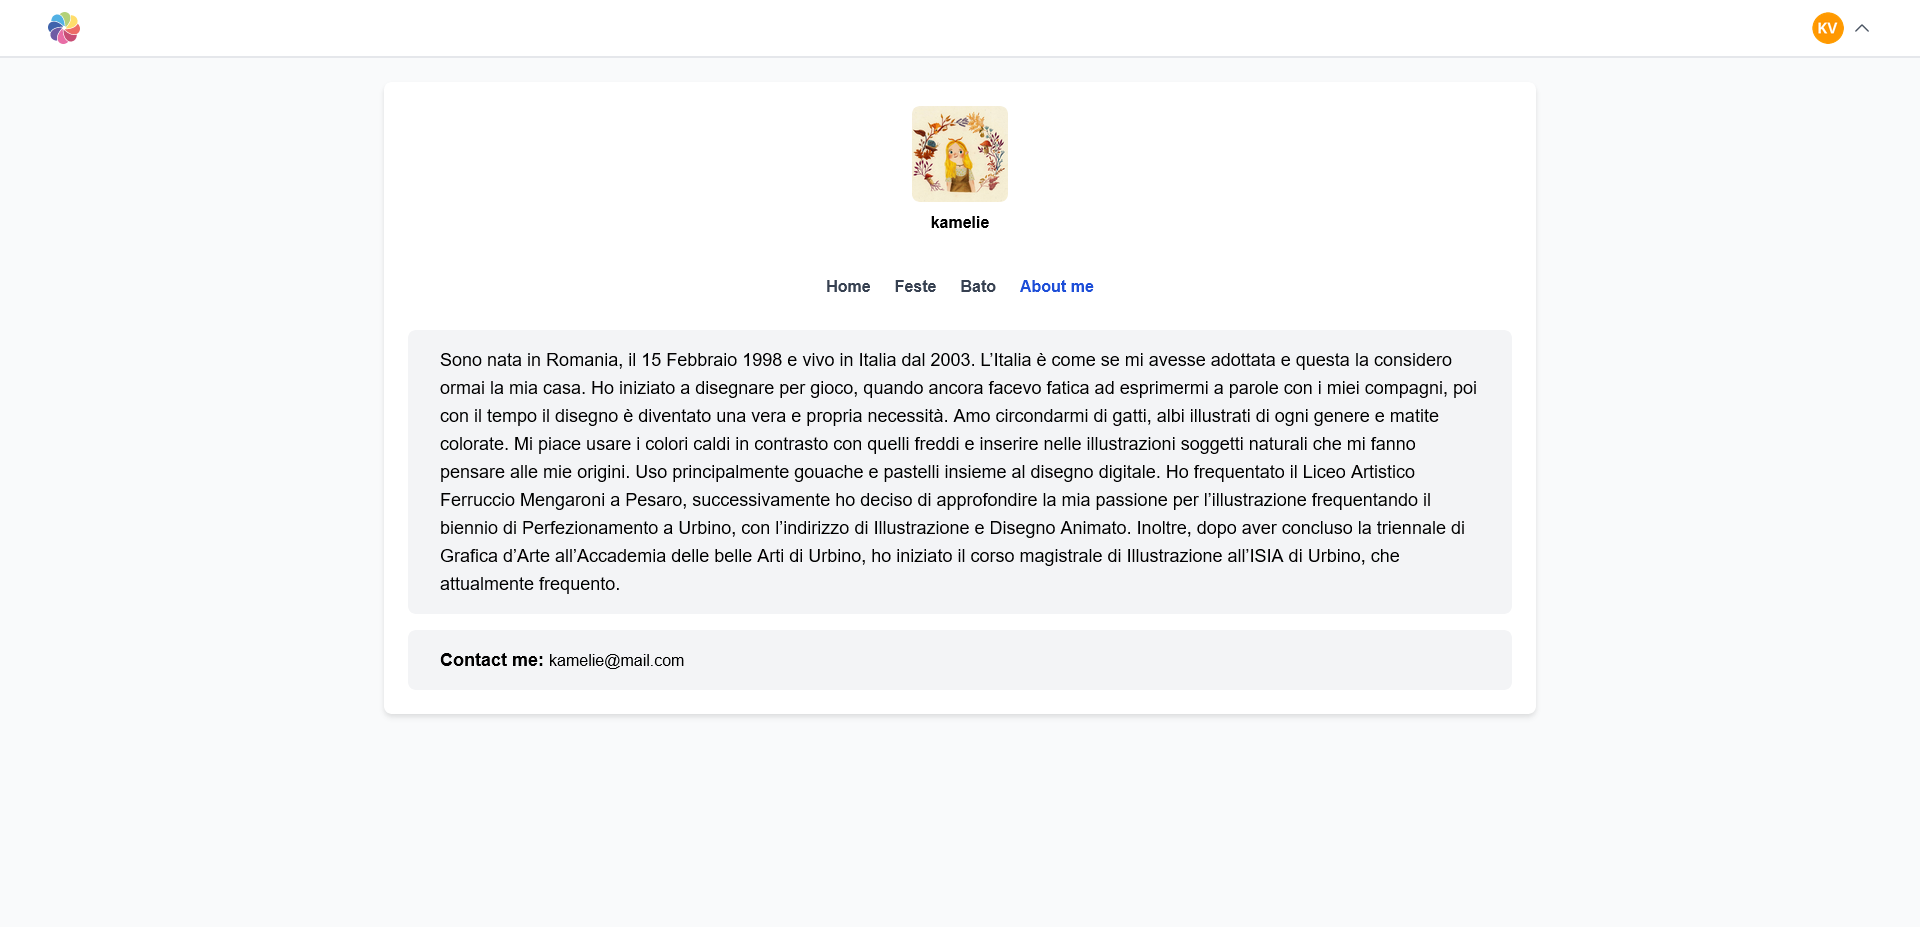
\includegraphics[width=1.0\linewidth]{figure/p-am-view}}
	\caption{Pagina ``about-me'' del portfolio pubblico}
	\label{fig:p-am-view}
\end{figure}

Durante il caricamento della pagina, viene eseguita la funzione \verb|setup()|, la quale verifica se nell'URL \`e presente lo slug di sezione. In tal caso, verifica la tipologia di sezione e se corrisponde a ,``about-me'' viene eseguito la funzione \verb|getAboutMe|. Tale funzione controlla se nello stato \verb|portfolio|, dello store Pinia \verb|PortfolioStore|, \`e presente l'attributo \verb|biography|. Se tale attributo non \`e presente, viene eseguita l'azione \verb|fetchAboutMe| che effettua una richiesta GET all'URI dell'API \verb|v1/portfolios/{portfolio}/about-me| per ottenere la biografia e il contatto

Se la richiesta ha successo la sezione verr\`a aggiunta alla lista \verb|sections| dello stato \verb|portfolio|.














